%Version 3.1 December 2024
% See section 11 of the User Manual for version history
%
%%%%%%%%%%%%%%%%%%%%%%%%%%%%%%%%%%%%%%%%%%%%%%%%%%%%%%%%%%%%%%%%%%%%%%
%%                                                                 %%
%% Please do not use \input{...} to include other tex files.       %%
%% Submit your LaTeX manuscript as one .tex document.              %%
%%                                                                 %%
%% All additional figures and files should be attached             %%
%% separately and not embedded in the \TeX\ document itself.       %%
%%                                                                 %%
%%%%%%%%%%%%%%%%%%%%%%%%%%%%%%%%%%%%%%%%%%%%%%%%%%%%%%%%%%%%%%%%%%%%%

%%\documentclass[referee,sn-basic]{sn-jnl}% referee option is meant for double line spacing

%%=======================================================%%
%% to print line numbers in the margin use lineno option %%
%%=======================================================%%

%%\documentclass[lineno,pdflatex,sn-basic]{sn-jnl}% Basic Springer Nature Reference Style/Chemistry Reference Style

%%=========================================================================================%%
%% the documentclass is set to pdflatex as default. You can delete it if not appropriate.  %%
%%=========================================================================================%%

%%\documentclass[sn-basic]{sn-jnl}% Basic Springer Nature Reference Style/Chemistry Reference Style

%%Note: the following reference styles support Namedate and Numbered referencing. By default the style follows the most common style. To switch between the options you can add or remove “Numbered” in the optional parenthesis. 
%%The option is available for: sn-basic.bst, sn-chicago.bst%  
 
%%\documentclass[pdflatex,sn-nature]{sn-jnl}% Style for submissions to Nature Portfolio journals
%%\documentclass[pdflatex,sn-basic]{sn-jnl}% Basic Springer Nature Reference Style/Chemistry Reference Style
% The float package is loaded before the class: the class loads hyperref, and a float package loaded
% after hyperref (by the algorithm package below) writes the anchor of every figure and algorithm twice.
\RequirePackage{float}
\documentclass[pdflatex,sn-mathphys-num]{sn-jnl}% Math and Physical Sciences Numbered Reference Style
%%\documentclass[pdflatex,sn-mathphys-ay]{sn-jnl}% Math and Physical Sciences Author Year Reference Style
%%\documentclass[pdflatex,sn-aps]{sn-jnl}% American Physical Society (APS) Reference Style
%%\documentclass[pdflatex,sn-vancouver-num]{sn-jnl}% Vancouver Numbered Reference Style
%%\documentclass[pdflatex,sn-vancouver-ay]{sn-jnl}% Vancouver Author Year Reference Style
%%\documentclass[pdflatex,sn-apa]{sn-jnl}% APA Reference Style
%%\documentclass[pdflatex,sn-chicago]{sn-jnl}% Chicago-based Humanities Reference Style

%%%% Standard Packages
%%<additional latex packages if required can be included here>
\usepackage[T1]{fontenc}

\usepackage{graphicx}%
\usepackage{multirow}%
\usepackage{amsmath,amssymb,amsfonts}%
\usepackage{amsthm}%
\usepackage{mathrsfs}%
\usepackage[title]{appendix}%
\usepackage{xcolor}%
\usepackage{textcomp}%
\usepackage{manyfoot}%
\usepackage{booktabs}%
\usepackage{algorithm}%
\usepackage{algorithmicx}%
\usepackage{algpseudocode}%
\usepackage{listings}%
%%%%
% References by \cref. With \newtheorem and a shared counter, \cref calls a lemma "Theorem" under this class,
% so the environments that share the counter of theorem are declared with thmtools below.
\usepackage{thmtools}%
\usepackage[capitalise,noabbrev]{cleveref}%

%%%%%=============================================================================%%%%
%%%%  Remarks: This template is provided to aid authors with the preparation
%%%%  of original research articles intended for submission to journals published 
%%%%  by Springer Nature. The guidance has been prepared in partnership with 
%%%%  production teams to conform to Springer Nature technical requirements. 
%%%%  Editorial and presentation requirements differ among journal portfolios and 
%%%%  research disciplines. You may find sections in this template are irrelevant 
%%%%  to your work and are empowered to omit any such section if allowed by the 
%%%%  journal you intend to submit to. The submission guidelines and policies 
%%%%  of the journal take precedence. A detailed User Manual is available in the 
%%%%  template package for technical guidance.
%%%%%=============================================================================%%%%

%% as per the requirement new theorem styles can be included as shown below
\theoremstyle{thmstyleone}%
\newtheorem{theorem}{Theorem}%  meant for continuous numbers
%%\newtheorem{theorem}{Theorem}[section]% meant for sectionwise numbers
%% optional argument [theorem] produces theorem numbering sequence instead of independent numbers for Proposition
%%\newtheorem{proposition}[theorem]{Proposition}%
%%\newtheorem{proposition}{Proposition}% to get separate numbers for theorem and proposition etc.
% Proposition, Lemma and Corollary are numbered with Theorem, in the style of Theorem.
\declaretheorem[name=Proposition, style=thmstyleone, sibling=theorem]{proposition}%
\declaretheorem[name=Lemma, style=thmstyleone, sibling=theorem]{lemma}%
\declaretheorem[name=Corollary, style=thmstyleone, sibling=theorem]{corollary}%

\theoremstyle{thmstyletwo}%
\newtheorem{example}{Example}%
\newtheorem{remark}{Remark}%

\theoremstyle{thmstylethree}%
\newtheorem{definition}{Definition}%

% Algorithm: the input and the output are headed "Input:" and "Output:".
\algrenewcommand\algorithmicrequire{\textbf{Input:}}%
\algrenewcommand\algorithmicensure{\textbf{Output:}}%

% Notation.
\newcommand{\cp}{\operatorname{cp}}% cp(u,v): number of edges of a minimum cut-path
\newcommand{\DC}{\mathcal{DC}_2}% graphs with distance or cut-value at most two
\newcommand{\MinCutPath}{\textsc{Min Cut-Path}}%
\newcommand{\SSP}{\textsc{Separating Shortest Path}}%
\newcommand{\PathInMinCut}{\textsc{Path in Min Cut}}%
\newcommand{\dn}{\mathord{\downarrow}}%
\newcommand{\upp}{\mathord{\uparrow}}%
\newcommand{\pos}{\mathrm{pos}}%
\newcommand{\MB}{\mathrm{MB}}%
\newcommand{\MA}{\mathrm{MA}}%
\newcommand{\Pos}{\mathrm{Pos}}%
\newcommand{\win}{\mathrm{win}}%
\newcommand{\FR}{\mathrm{FR}}%
\newcommand{\ER}{\mathrm{ER}}%
\newcommand{\EP}{\mathrm{EP}}%

% Title and author of the PDF file.
\hypersetup{pdftitle={Min Cut-Path: NP-Complete on Diameter Three, Polynomial for Distance or Cut-Value Two}, pdfauthor={Norbert Miche\v{l}}}%

\raggedbottom
%%\unnumbered% uncomment this for unnumbered level heads

\begin{document}

\title{Min Cut-Path: NP-Complete on Diameter Three, Polynomial for Distance or Cut-Value Two}

\author*{\fnm{Norbert} \sur{Miche\v{l}}}\email{5344553@upjs.sk}

\affil{\orgdiv{Institute of Computer Science, Faculty of Science}, \orgname{Pavol Jozef \v{S}af\'arik University in Ko\v{s}ice}, \orgaddress{\street{Jesenn\'a 5}, \city{Ko\v{s}ice}, \postcode{040 01}, \country{Slovakia}}}

%%==================================%%
%% Sample for unstructured abstract %%
%%==================================%%

\abstract{A cut-path between two vertices $u$ and $v$ of a graph is a set of edges that contains both a $u$--$v$ path and a cut separating $u$ from $v$.
The \MinCutPath{} problem asks for a cut-path with the fewest edges.
Let $d(u,v)$ be the distance between $u$ and $v$, and let the cut-value $c(u,v)$ be the size of a minimum cut separating them.
We prove that \MinCutPath{} is NP-complete on graphs of diameter three, already for pairs with $d(u,v) = 2$.
We then prove that it is solvable in polynomial time on the graphs in which every two vertices are at distance at most two or have cut-value at most two.
This class contains the graphs of diameter two and the cactus graphs.
For a pair with cut-value two, the minimum cuts divide the graph into a chain of subgraphs.
A minimum cut-path has $d(u,v)$ edges if and only if one of these subgraphs contains a path that lies on a shortest $u$--$v$ path, joins two of the four terminals of the subgraph and separates the other two.
In the class, this gives a linear-time algorithm.
An adjacent pair takes one minimum cut.
The remaining pairs have $d(u,v) = 2$ and $c(u,v) \geq 3$, and there a minimum cut-path has $c(u,v)$ edges if and only if some minimum cut contains a $u$--$v$ path.
The minimum cuts are the down-sets of a preorder, and the condition on distances gives every two incomparable elements a common neighbor below both or above both.
We show that a bounded number of elements determines a down-set whose cut contains a given shortest solution, and enumeration of these descriptions decides the question.}

%%================================%%
%% Sample for structured abstract %%
%%================================%%

% \abstract{\textbf{Purpose:} The abstract serves both as a general introduction to the topic and as a brief, non-technical summary of the main results and their implications. The abstract must not include subheadings (unless expressly permitted in the journal's Instructions to Authors), equations or citations. As a guide the abstract should not exceed 200 words. Most journals do not set a hard limit however authors are advised to check the author instructions for the journal they are submitting to.
% 
% \textbf{Methods:} The abstract serves both as a general introduction to the topic and as a brief, non-technical summary of the main results and their implications. The abstract must not include subheadings (unless expressly permitted in the journal's Instructions to Authors), equations or citations. As a guide the abstract should not exceed 200 words. Most journals do not set a hard limit however authors are advised to check the author instructions for the journal they are submitting to.
% 
% \textbf{Results:} The abstract serves both as a general introduction to the topic and as a brief, non-technical summary of the main results and their implications. The abstract must not include subheadings (unless expressly permitted in the journal's Instructions to Authors), equations or citations. As a guide the abstract should not exceed 200 words. Most journals do not set a hard limit however authors are advised to check the author instructions for the journal they are submitting to.
% 
% \textbf{Conclusion:} The abstract serves both as a general introduction to the topic and as a brief, non-technical summary of the main results and their implications. The abstract must not include subheadings (unless expressly permitted in the journal's Instructions to Authors), equations or citations. As a guide the abstract should not exceed 200 words. Most journals do not set a hard limit however authors are advised to check the author instructions for the journal they are submitting to.}

\keywords{Separating shortest path, Edge connectivity, Minimum cuts, Graph diameter, NP-completeness}

%%\pacs[JEL Classification]{D8, H51}

%%\pacs[MSC Classification]{35A01, 65L10, 65L12, 65L20, 65L70}

\maketitle

\section{Introduction}\label{sec:introduction}

Let $G$ be a connected graph, and let $u$ and $v$ be two distinct vertices of $G$.
A \emph{cut-path} between $u$ and $v$ is a set of edges that contains a $u$--$v$ path and a cut separating $u$ from $v$.
The \MinCutPath{} problem asks for a cut-path with the fewest edges, and $\cp(u, v)$ denotes their number.
Let $d(u, v)$ be the distance between $u$ and $v$, and let the cut-value $c(u, v)$ be the minimum number of edges of a cut separating $u$ from $v$.
By~\cite[Lemma~2.3]{Michel2026MinCutPath},
\[
\max\{c(u, v), d(u, v)\} \leq \cp(u, v) \leq c(u, v) + d(u, v) - 1.
\]

The \MinCutPath{} problem was introduced in the author's master's thesis~\cite{Michel2025MinCutPath}.
The upper bound is attained by all pairs of vertices in graphs of diameter two and in cactus graphs~\cite[Theorems~5.5 and~6.2]{Michel2026MinCutPath}, where the cactus graphs are the connected graphs with $c(x, y) \leq 2$ for all pairs $x, y$ (\cref{sec:class}).
A shortest $u$--$v$ path is separating if the removal of its edges separates $u$ from $v$, and $\cp(u, v) = d(u, v)$ if and only if such a path exists.
Deciding whether it exists, the \SSP{} problem, is NP-complete~\cite[Theorem~3.10]{Michel2026MinCutPath}.

The formula $\cp(u, v) = c(u, v) + d(u, v) - 1$ fails if every pair of vertices is required to satisfy only one of the two hypotheses.
Let $\DC$ be the class of connected graphs in which every two distinct vertices $x$ and $y$ satisfy $d(x, y) \leq 2$ or $c(x, y) \leq 2$.
The thesis defines this class and gives two graphs in it with $\cp(u, v) = 3$ and $c(u, v) + d(u, v) - 1 = 4$~\cite[Definition~37 and Figure~3.3]{Michel2025MinCutPath}.
We prove that \MinCutPath{} is NP-complete on graphs of diameter three and solvable in polynomial time on $\DC$.

\subsection{Our Results}\label{sec:results}

\begin{enumerate}
\item \emph{NP-completeness on diameter three.}
Deciding whether $\cp(u, v) = c(u, v)$ is NP-complete on graphs of diameter three, already for pairs with $d(u, v) = 2$.
Hence the decision version of \MinCutPath{} is NP-complete on these graphs, and deciding whether $\cp(u, v) = c(u, v) + d(u, v) - 1$ is coNP-complete (\cref{thm:dt-hardness,cor:dt-consequences}).

\item \emph{Pairs of $\DC$ with cut-value at most two.}
Let $c(u, v) = 2$ in an arbitrary connected graph.
The minimum $u$--$v$ cuts divide the graph into a chain of subgraphs, the squares (\cref{thm:structure}).
We have $\cp(u, v) = d(u, v)$ if and only if some square contains a path from an entering to a leaving terminal that lies on a shortest $u$--$v$ path and separates the other two terminals (\cref{thm:characterization}).
For a graph $G = (V, E)$ of $\DC$, this gives an $O(|V| + |E|)$ algorithm for $\cp(u, v)$ and a minimum cut-path (\cref{thm:linear-time,cor:class-pairs}).

\item \emph{Pairs of $\DC$ at distance two.}
A pair with $d(u, v) = 1$ is solved by one minimum cut, and the other pairs of $\DC$ that item 2 leaves have $d(u, v) = 2$ and $c(u, v) \geq 3$ (\cref{prop:easy-pairs}).
For these, $\cp(u, v) \in \{c(u, v), c(u, v) + 1\}$, and $\cp(u, v) = c(u, v)$ if and only if some minimum $u$--$v$ cut contains a $u$--$v$ path (\cref{prop:open-pairs}).
We decide this question and construct a minimum cut-path in $O(n^{30})$ time for $n = |V|$ (\cref{thm:pa-open-case}).
\end{enumerate}

Items 2 and 3 together give our main result.

\begin{theorem}\label{thm:main}
\MinCutPath{} restricted to the graphs of $\DC$ is solvable in polynomial time.
\end{theorem}

\begin{proof}
A pair with $d(u, v) = 1$, or with $c(u, v) \leq 2$, is solved by \cref{thm:linear-time,cor:class-pairs}.
A pair with $d(u, v) \geq 3$ has $c(u, v) \leq 2$ by the definition of $\DC$.
Every other pair has $d(u, v) = 2$ and $c(u, v) \geq 3$ and is solved by \cref{thm:pa-open-case}.
\end{proof}

\subsection{Techniques}\label{sec:techniques}

The hardness proof reduces from 3-SAT.
Two cliques force every minimum $u$--$v$ cut to correspond to an assignment of the variables, and $u$ and $v$ are connected by the edges of the cut if and only if the assignment satisfies the formula.

For $c(u, v) = 2$, consecutive squares are joined by two general paths, and a $u$--$v$ path $R$ follows exactly one of them.
Hence $u$ and $v$ are separated in $G \setminus R$ if and only if, in some square, the part of $R$ in the square separates the two terminals at the edges of the square that $R$ does not use (\cref{lem:criterion}).
In a graph of $\DC$, such a part of a shortest path has at most two edges (\cref{cor:two-edges}), which leaves a constant number of candidates per square.

For $d(u, v) = 2$ and $c(u, v) \geq 3$, the minimum cuts are the down-sets of a preorder (Picard and Queyranne~\cite{PicardQueyranne1980}), and a path in a minimum cut alternates between the two sides.
The hypothesis $G \in \DC$ gives two incomparable elements of the preorder a common neighbor below both or above both (\cref{thm:zz-reduction}).
A solution is a shortest walk $P$ that alternates between the two sides of some down-set.
It suffices to separate the minimal elements $A_P$ that $P$ uses on the upper side from the maximal elements $B_P$ that it uses on the lower side.
Two far-apart members of $A_P$, or of $B_P$, determine a down-set that separates all but few pairs, because an element that met two far-apart members would shorten $P$.
A formula of unions and intersections over at most $28$ elements then gives a down-set that contains the solution (\cref{thm:pa-formulas}), and the algorithm tries all such formulas.

\subsection{Related Work}\label{sec:related-work}

By Menger's theorem, $c(u, v)$ is the maximum number of pairwise edge-disjoint $u$--$v$ paths~\cite[Corollary~3.3.5]{Diestel2025}.
Picard and Queyranne~\cite{PicardQueyranne1980} described all minimum cuts between two vertices of a network by one maximum flow.
A set that contains the source and not the sink is the source side of a minimum cut if and only if no arc of the residual digraph leaves it.
For an undirected graph, contract every class of vertices that no minimum $u$--$v$ cut separates and direct the remaining edges along a maximum flow.
The result is an acyclic digraph in which every vertex other than the classes of $u$ and $v$ has as many entering as leaving edges, a structure that Dinitz and Vainshtein call a strip (see~\cite{BaswanaPandey2025Carcass}).
All minimum cuts of a graph are represented by a cactus, a result of Dinits, Karzanov and Lomonosov (see~\cite{NagamochiKameda1996}).
For a 2-edge-connected graph that is not 3-edge-connected, this cactus is obtained by contracting every 3-edge-connected component, that is, every class of the relation $c(x, y) \geq 3$, and it is computed in linear time~\cite{Mehlhorn2017Certifying}.
For a pair with $c(u, v) = 2$, the square decomposition of \cref{sec:structure} is an explicit form of these representations.
We prove its properties directly, because \cref{sec:separating,sec:algorithm} use the terminals of the squares and distances inside the squares, which a contraction does not keep.

A $u$--$v$ path is non-disconnecting if the removal of its edges leaves the graph connected.
Deciding whether such a path exists is NP-hard~\cite{Mao2021NonSeparating}, and a shortest one is found in FPT time with respect to its length~\cite{Abhinav2022NonSeparating}.
For two pairs of vertices, it is NP-complete to decide whether some shortest path between the first pair is edge-disjoint from some path between the second pair~\cite{EilamTzoreff1998Disjoint}.
\SSP{} asks the opposite, namely whether the removal of the edges of some shortest $u$--$v$ path separates $u$ from $v$.

Graphs in which the local edge-connectivity $c(x, y)$ of every pair of vertices is at most a constant $k$ were studied for coloring problems~\cite{Aboulker2017Coloring}.
For $k = 2$ the connected graphs of this kind are the cactus graphs.
The class $\DC$ asks for $c(x, y) \leq 2$ only when $d(x, y) \geq 3$, so it contains all cactus graphs and all connected graphs of diameter two.
To the best of our knowledge, a class defined by such a condition on distances and cut-values has not been studied.
Graphs of diameter two are also a polynomial case of \textsc{Matching Cut} and, for unit edge lengths, of \textsc{Shortest Path Most Vital Edges}, and both problems are NP-hard on graphs of diameter three~\cite{LeLe2019MatchingCut,Bazgan2019MostVital}.

\subsection{Relation to the Thesis}\label{sec:thesis}

Section~3.3 of the thesis~\cite[Definitions~37 to~40 and Theorems~20, 22 and~23]{Michel2025MinCutPath} contains the class $\DC$, the two graphs of \cref{ex:counterexamples} and the notions of a square and of a general path.
It also contains the idea of a polynomial and of a linear-time algorithm for pairs with cut-value two.
The thesis obtains a decomposition by three transformations of the graph.
Here the decomposition is defined by the union of all minimum $u$--$v$ cuts, and every statement on it has a complete proof.
The separation criterion and the characterization for arbitrary graphs (\cref{lem:criterion,thm:characterization}), the linear running time that includes the computation of the decomposition (\cref{thm:linear-time}), and \cref{sec:dt-diameter-three,sec:zz-zigzag,sec:pa-polynomial} are new.

\section{Preliminaries}
\label{sec:preliminaries}

\subsection{Cut-Paths and Minimum Cuts}
\label{sec:cut-paths}

All graphs are finite, simple and undirected.
Notions that are not defined here follow~\cite{Diestel2025}.
Throughout the paper, $G = (V, E)$ is a connected graph, and $u$ and $v$ are two distinct vertices of $G$.
We write $xy$ for the edge with the ends $x$ and $y$.
A path is a sequence of distinct vertices in which consecutive vertices are adjacent, and a single vertex is a path with no edges.
A path from $x$ to $y$ is an $x$--$y$ path.
We write $|P|$ for the number of edges of a path $P$ and use the symbol $P$ also for the set of its edges.
The distance $d(x, y)$ is the number of edges of a shortest $x$--$y$ path of $G$.
For a subgraph $H$ of $G$ and a set $M \subseteq E$, the graph $H \setminus M$ is obtained from $H$ by removing the edges of $M$.

Let $x$ and $y$ be two distinct vertices.
A set $C \subseteq E$ is an \emph{$x$--$y$ cut} if $G \setminus C$ contains no $x$--$y$ path.
The minimum size of an $x$--$y$ cut is the \emph{cut-value} $c(x, y)$.
For a set $A \subseteq V$, we denote by $\delta(A)$ the set of all edges with exactly one end in $A$.
If $x \in A$ and $y \notin A$, then $\delta(A)$ is an $x$--$y$ cut.
Distances and cut-values in a subgraph $H$ are written $d_H$ and $c_H$.

\begin{definition}[Cut-path]
\label{def:cut-path}
A \emph{cut-path} between $u$ and $v$ is a set of edges of $G$ that contains a $u$--$v$ path and a $u$--$v$ cut.
The minimum number of edges of a cut-path between $u$ and $v$ is denoted by $\cp(u, v)$, and a cut-path with $\cp(u, v)$ edges is a \emph{minimum cut-path}.
\end{definition}

The \MinCutPath{} problem asks for a minimum cut-path between $u$ and $v$.
A shortest $u$--$v$ path $P$ is \emph{separating} if $G \setminus P$ contains no $u$--$v$ path, and the \SSP{} problem asks whether $G$ contains such a path.

\begin{lemma}[{\cite[Lemma~2.3 and its proof, and the proof of Theorem~3.11]{Michel2026MinCutPath}}]
\label{lem:basic-bounds}
The value $\cp(u, v)$ satisfies
\[
\max\{c(u, v), d(u, v)\} \leq \cp(u, v) \leq c(u, v) + d(u, v) - 1,
\]
and the union of a minimum $u$--$v$ cut and a shortest $u$--$v$ path is a cut-path with at most $c(u, v) + d(u, v) - 1$ edges.
The equality $\cp(u, v) = d(u, v)$ holds if and only if $G$ contains a separating shortest $u$--$v$ path.
\end{lemma}

\begin{lemma}
\label{lem:minimum-cuts}
Let $C$ be a minimum $u$--$v$ cut.
Then $G \setminus C$ has exactly two components, and $C = \delta(A)$ for exactly one set $A \subseteq V$ with $u \in A$, the vertex set of the component that contains $u$.
For every set $A \subseteq V$ with $u \in A$ and $v \notin A$, every $u$--$v$ path contains an odd number of edges of $\delta(A)$~\cite[Lemma~5.4]{Michel2026MinCutPath}.
\end{lemma}

\begin{proof}
Let $A$ be the vertex set of the component of $G \setminus C$ that contains $u$.
Every edge of $\delta(A)$ belongs to $C$, and $\delta(A)$ is a $u$--$v$ cut because $v \notin A$.
Hence $\delta(A) = C$ by the minimality of $C$.
Let $Y$ be the component of $G \setminus C$ that contains $v$, and suppose that there is a third component $Y'$.
Since $G$ is connected, some edge of $G$ has exactly one end in $Y'$.
This edge belongs to $C = \delta(A)$ and has no end in $Y$.
The edges of $C$ with an end in $Y$ thus form a $u$--$v$ cut with fewer than $|C|$ edges, a contradiction.
If $C = \delta(A')$ for a set $A'$ with $u \in A'$, then no edge of $G \setminus C$ has exactly one end in $A'$, so $A'$ is the union of the vertex sets of some components of $G \setminus C$.
Since $\delta(V)$ is empty and $C$ is not, we have $A' \neq V$ and hence $A' = A$.
\end{proof}

When we write a minimum $u$--$v$ cut as $\delta(A)$, the set $A$ contains $u$.

\begin{lemma}
\label{lem:uncrossing}
Let $A, B \subseteq V$, and let $m(A, B)$ be the number of edges with one end in $A \setminus B$ and the other end in $B \setminus A$.
Then
\[
|\delta(A \cap B)| + |\delta(A \cup B)| = |\delta(A)| + |\delta(B)| - 2m(A, B).
\]
\end{lemma}

\begin{proof}
The sets $A \cap B$, $A \setminus B$, $B \setminus A$ and $V \setminus (A \cup B)$ partition $V$.
An edge with both ends in one of them is counted on neither side.
An edge between $A \setminus B$ and $B \setminus A$ belongs to $\delta(A)$ and to $\delta(B)$ and to neither set on the left-hand side.
An edge between $A \cap B$ and $V \setminus (A \cup B)$ belongs to all four sets.
Every other edge belongs to exactly one of $\delta(A)$, $\delta(B)$ and to exactly one of $\delta(A \cap B)$, $\delta(A \cup B)$.
\end{proof}

The inequality $|\delta(A \cap B)| + |\delta(A \cup B)| \leq |\delta(A)| + |\delta(B)|$ is the submodularity of the cut function.

\begin{proposition}
\label{prop:open-pairs}
Let $G$ be a connected graph and let $u, v$ be two distinct vertices of $G$.
Then $\cp(u, v) = c(u, v)$ if and only if some minimum $u$--$v$ cut contains a $u$--$v$ path.
Such a path has an odd number of edges, and at least three edges if $d(u, v) = 2$.
\end{proposition}

\begin{proof}
A minimum $u$--$v$ cut that contains a $u$--$v$ path is a cut-path with $c(u, v)$ edges, and $\cp(u, v) \geq c(u, v)$ by \cref{lem:basic-bounds}.
Conversely, a cut-path with $c(u, v)$ edges contains a $u$--$v$ cut, which has at least $c(u, v)$ edges.
The cut-path is therefore equal to this cut, so it is a minimum $u$--$v$ cut, and it contains a $u$--$v$ path.
A minimum $u$--$v$ cut is $\delta(A)$ for a set $A$ with $u \in A$ and $v \notin A$, and a $u$--$v$ path contained in $\delta(A)$ has an odd number of edges by \cref{lem:minimum-cuts}.
If $d(u, v) = 2$, the path has at least two edges, hence at least three.
\end{proof}

In the graph $G_b$ of \cref{ex:counterexamples}, the minimum $u$--$v$ cut $\delta(\{u, s, b\}) = \{ua, ab, bv\}$ is the path $u, a, b, v$.
In a graph of diameter two, $\cp(u, v) = c(u, v) + 1$ for every pair with $d(u, v) = 2$~\cite[Theorem~5.5]{Michel2026MinCutPath}, so by \cref{prop:open-pairs} no minimum $u$--$v$ cut contains a $u$--$v$ path.

\subsection{Graphs with Distance or Cut-Value at Most Two}
\label{sec:class}

\begin{definition}[The class $\DC$, {\cite[Definition~37]{Michel2025MinCutPath}}]
\label{def:class}
The class $\DC$ consists of all connected graphs in which every two distinct vertices $x$ and $y$ satisfy $d(x, y) \leq 2$ or $c(x, y) \leq 2$.
\end{definition}

A graph has \emph{diameter at most two} if any two of its vertices are at distance at most two.
A \emph{cactus graph} is a connected graph in which any two distinct cycles share at most one vertex.
The cactus graphs are the connected graphs in which $c(x, y) \leq 2$ for every two distinct vertices $x$ and $y$~\cite[Lemma~6.1]{Michel2026MinCutPath}.

\begin{proposition}
\label{prop:class}
The relation on $V$ that holds for $x$ and $y$ if $x = y$ or $c(x, y) \geq 3$ is an equivalence relation.
The graph $G$ belongs to $\DC$ if and only if any two vertices of the same equivalence class are at distance at most two in $G$.
In particular, $\DC$ contains all connected graphs of diameter at most two and all cactus graphs.
\end{proposition}

\begin{proof}
The relation is reflexive and symmetric.
For transitivity, let $x, y, z$ be distinct vertices with $c(x, y) \geq 3$ and $c(y, z) \geq 3$, and let $C$ be a minimum $x$--$z$ cut.
If $y$ lies in the component of $G \setminus C$ that contains $x$, then $C$ is a $y$--$z$ cut, and otherwise $C$ is an $x$--$y$ cut.
In both cases $|C| \geq 3$.
By \cref{def:class}, the graph $G$ lies outside $\DC$ if and only if some two distinct vertices $x, y$ satisfy $c(x, y) \geq 3$ and $d(x, y) \geq 3$, which is the second statement.
In a graph of diameter at most two all distances are at most two, and in a cactus graph every equivalence class is a single vertex.
\end{proof}

The equivalence classes of \cref{prop:class} are called 3-edge-connected components in~\cite{Mehlhorn2017Certifying}, where they are computed in linear time.
Hence membership in $\DC$ is tested in polynomial time.

In graphs of diameter at most two and in cactus graphs, every pair satisfies $\cp(u, v) = c(u, v) + d(u, v) - 1$~\cite[Theorems~5.5 and~6.2]{Michel2026MinCutPath}.
\Cref{fig:graph-classes} shows the three classes.
The formula fails in $\DC$, as the two graphs of~\cite[Figure~3.3]{Michel2025MinCutPath} show (\cref{ex:counterexamples}).

\begin{figure}[tb]
    \centering
    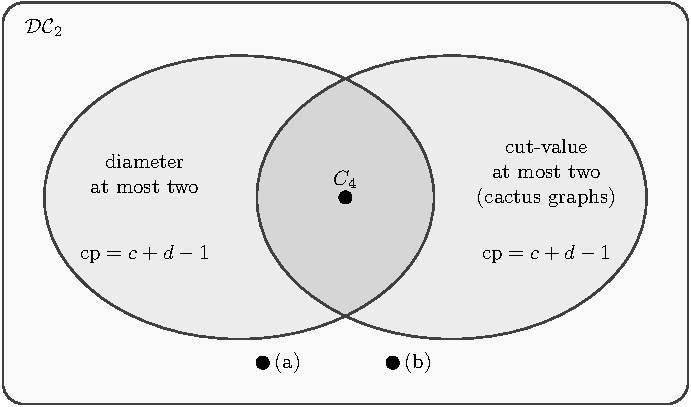
\includegraphics{graph-classes.pdf}
    \caption{The class $\DC$ and its two subclasses; (a) and (b) are the graphs $G_a$ and $G_b$ of \cref{fig:counterexamples}}
    \label{fig:graph-classes}
\end{figure}

\begin{example}
\label{ex:counterexamples}
Let $G_a$ be the graph with the vertices $u, v, a, b, s, t$ and the edges $ua$, $us$, $sb$, $ab$, $at$, $tv$, $bv$, and let $G_b$ be obtained from $G_a$ by adding the edges $av$ and $ub$ (\cref{fig:counterexamples}).
In both graphs, the removal of the path $u, a, b, v$ leaves the components $\{u, s, b\}$ and $\{a, t, v\}$, so this path is a cut-path with three edges.
In $G_a$ we have $c(u, v) = 2$ and $d(u, v) = 3$, and in $G_b$ we have $c(u, v) = 3$ and $d(u, v) = 2$.
Hence $\cp(u, v) = 3$ in both graphs by \cref{lem:basic-bounds}, whereas $c(u, v) + d(u, v) - 1 = 4$.
Both graphs belong to $\DC$.
In $G_a$ the only two vertices of degree greater than two are $a$ and $b$, which are adjacent.
In $G_b$ the only two vertices at distance three are $s$ and $t$, which have degree two.
Neither graph has diameter two, and neither is a cactus graph.
\end{example}

\begin{figure}[tb]
    \centering
    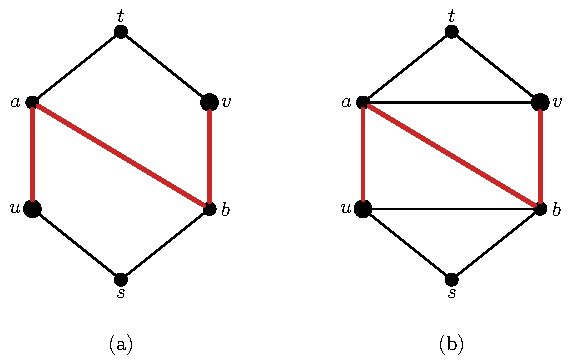
\includegraphics{counterexamples.pdf}
    \caption{The graphs $G_a$ (a) and $G_b$ (b) of \cref{ex:counterexamples}; the cut-path $u, a, b, v$ is red}
    \label{fig:counterexamples}
\end{figure}

\begin{proposition}
\label{prop:easy-pairs}
(i) If $d(u, v) = 1$, then $\cp(u, v) = c(u, v)$, and every minimum $u$--$v$ cut is a minimum cut-path.
(ii) If $c(u, v) = 1$, then $\cp(u, v) = d(u, v)$, and every shortest $u$--$v$ path is a minimum cut-path.
(iii) If $c(u, v) = 2$, then $\cp(u, v) \in \{d(u, v), d(u, v) + 1\}$.
(iv) If $d(u, v) = 2$, then $\cp(u, v) \in \{c(u, v), c(u, v) + 1\}$.
If $G \in \DC$, then $d(u, v) \leq 2$ or $c(u, v) \leq 2$, so at least one of the four statements applies to every pair $u, v$.
\end{proposition}

\begin{proof}
The four values follow from \cref{lem:basic-bounds}.
If $d(u, v) = 1$, the edge $uv$ is a $u$--$v$ path and lies in every $u$--$v$ cut, so every minimum $u$--$v$ cut is a cut-path.
If $c(u, v) = 1$, the edge of a $u$--$v$ cut of size one lies on every $u$--$v$ path, so every shortest $u$--$v$ path is a cut-path.
The last statement is \cref{def:class}.
\end{proof}

By \cref{prop:easy-pairs}, a minimum cut-path in a graph of $\DC$ remains to be found for the pairs with $c(u, v) = 2$ and for the pairs with $d(u, v) = 2$ and $c(u, v) \geq 3$.
\Cref{sec:structure,sec:separating,sec:algorithm} treat the first kind.
\Cref{sec:zz-zigzag,sec:pa-polynomial} treat the second kind.

\section{NP-Completeness on Graphs of Diameter Three}
\label{sec:dt-diameter-three}

By \cref{prop:open-pairs}, $\cp(u, v) = c(u, v)$ if and only if some minimum $u$--$v$ cut contains a $u$--$v$ path.
The problem \PathInMinCut{} has as input a connected graph $G$ and two distinct vertices $u$ and $v$, and it asks whether some minimum $u$--$v$ cut of $G$ contains a $u$--$v$ path.
We prove that \PathInMinCut{} is NP-complete on graphs of diameter three, already for pairs at distance two (\cref{thm:dt-hardness}), and we draw the consequences for \MinCutPath{} (\cref{cor:dt-consequences}).

\subsection{The Reduction from 3-SAT}
\label{sec:dt-construction}

The reduction assigns to a formula $\varphi$ a graph $G_\varphi$ whose minimum $u$--$v$ cuts correspond to the truth assignments of $\varphi$ (\cref{lem:dt-cuts}).
The cut of an assignment contains a $u$--$v$ path if and only if the assignment satisfies $\varphi$ (\cref{lem:dt-cut-graphs}).

\begin{definition}[The graph $G_\varphi$]
\label{def:dt-graph}
Let $\varphi$ be a formula in conjunctive normal form with the clauses $C_1, \dots, C_m$, where $m \geq 1$, over the variables $x_1, \dots, x_p$.
A clause is a nonempty list of literals that may contain repetitions, a literal is a variable or a negated variable, and every variable occurs in some clause.
If every clause has three literals, then $\varphi$ is an instance of 3-SAT.
A \emph{truth assignment} $\tau$ sets every variable to true or to false, and $\tau$ \emph{satisfies} $\varphi$ if every clause contains a literal that is true under $\tau$.
Let $L$ be the total number of literals in the $m$ clauses, counted with repetitions, and let $c_0 = (m + 1) + 2L$ and $N = c_0 + 2$.

The vertex set of $G_\varphi$ consists of two disjoint sets $K^u$ and $K^v$ with $N$ vertices each and of the \emph{occurrence vertices} $o_{k,j}$, one for the $j$-th literal of $C_k$, for all $k$ and $j$.
Any two vertices of $K^u$ are adjacent, and so are any two vertices of $K^v$.
The clique $K^u$ contains the vertices $u = u_0, u_1, \dots, u_m$ and two \emph{anchors} $w_1, w_2$, and the clique $K^v$ contains the vertices $v_0, v_1, \dots, v_m = v$ and two anchors $z_1, z_2$.
Since $N - (m + 3) = 2L \geq 2$, each clique has $2L$ further vertices, its \emph{fillers}.
The \emph{rungs} $u_k v_k$, for $0 \leq k \leq m$, are the only edges between $K^u$ and $K^v$.
If the $j$-th literal of $C_k$ is a variable, then $o_{k,j}$ is a \emph{positive} occurrence vertex, adjacent to $v_{k-1}$, $v_k$, $w_1$ and $w_2$.
If this literal is a negated variable, then $o_{k,j}$ is a \emph{negative} occurrence vertex, adjacent to $u_{k-1}$, $u_k$, $z_1$ and $z_2$.
For every variable $x_i$, let $O_i$ be the set of the occurrence vertices of the literals $x_i$ and $\neg x_i$.
The vertices of $O_i$ are joined, in an arbitrary order, into a path by $|O_i| - 1$ \emph{synchronization edges}.
The graph $G_\varphi$ has no further edges.
For a truth assignment $\tau$, let $A_\tau$ be the union of $K^u$ and of all sets $O_i$ such that $\tau$ sets $x_i$ to true.
\end{definition}

\Cref{fig:dt-construction} shows $G_\varphi$ for $\varphi = (x_1 \vee \neg x_2) \wedge x_2$.

\begin{figure}[tb]
    \centering
    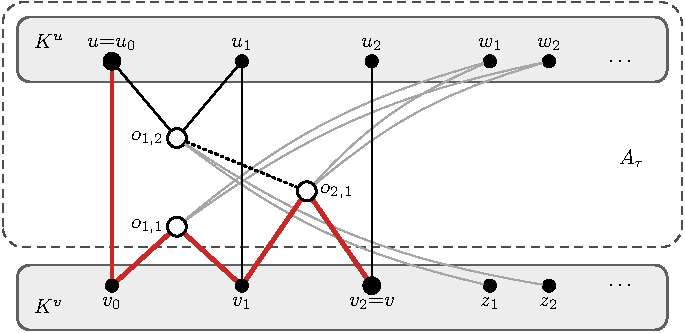
\includegraphics{hardness-construction.pdf}
    \caption{The graph $G_\varphi$ for $\varphi = (x_1 \vee \neg x_2) \wedge x_2$ without the clique edges and with a $u$--$v$ path in $\delta(A_\tau)$ for $\tau(x_1) = \tau(x_2) = \text{true}$ in red}
    \label{fig:dt-construction}
\end{figure}

Every occurrence vertex has exactly two neighbors in $K^u$ and two neighbors in $K^v$, and a filler has no neighbor outside its clique.
The graph $G_\varphi$ is connected, because the rungs join the two cliques and every occurrence vertex has a neighbor in a clique.
It has $2N + L$ vertices and $N(N - 1) + (m + 1) + 4L + (L - p)$ edges, where the four terms count the edges inside the cliques, the rungs, the edges at the occurrence vertices and the synchronization edges.
Hence $G_\varphi$ is computed in time polynomial in the length of $\varphi$.

\subsection{Minimum Cuts and Cut Graphs}
\label{sec:dt-correctness}

By \cref{lem:minimum-cuts}, every minimum $u$--$v$ cut is $\delta(A)$ for exactly one set $A$ with $u \in A$ and $v \notin A$.

\begin{lemma}[Forcing]
\label{lem:dt-forcing}
Let $G = (V, E)$ be the graph $G_\varphi$ of a formula $\varphi$ (\cref{def:dt-graph}).
Then $c(u, v) \leq c_0$, and every minimum $u$--$v$ cut $\delta(A)$ with $u \in A$ satisfies $K^u \subseteq A$ and $A \cap K^v = \emptyset$.
\end{lemma}

\begin{proof}
The edges that leave $K^u$ are the $m + 1$ rungs and the two edges from each of the $L$ occurrence vertices to $K^u$.
Hence $|\delta(K^u)| = c_0$, and $\delta(K^u)$ is a $u$--$v$ cut, so $c(u, v) \leq c_0$.
Let $\delta(A)$ be a minimum $u$--$v$ cut with $u \in A$, and suppose that some vertex $a \in K^u$ is not in $A$.
The edge $ua$ and the paths $u, y, a$ for $y \in K^u \setminus \{u, a\}$ are $N - 1$ edge-disjoint $u$--$a$ paths.
Each of them contains an edge of $\delta(A)$, because $u \in A$ and $a \notin A$.
Hence $|\delta(A)| \geq N - 1 = c_0 + 1 > c(u, v)$, a contradiction.
If some vertex $b \in K^v$ were in $A$, the $N - 1$ edge-disjoint $v$--$b$ paths in the clique $K^v$ would give the same contradiction, because $v \notin A$.
\end{proof}

\begin{lemma}[Minimum cuts]
\label{lem:dt-cuts}
Let $G = (V, E)$ be the graph $G_\varphi$ of a formula $\varphi$ with the variables $x_1, \dots, x_p$.
(i) Let $A$ be a set with $K^u \subseteq A \subseteq V \setminus K^v$, and let $k(A)$ be the number of synchronization edges in $\delta(A)$.
Then $\delta(A)$ consists of the $m + 1$ rungs, of two edges at every occurrence vertex $o$, which are the edges from $o$ to $K^v$ if $o \in A$ and the edges from $o$ to $K^u$ otherwise, and of the synchronization edges with exactly one end in $A$.
In particular, $|\delta(A)| = c_0 + k(A)$.
(ii) We have $c(u, v) = c_0$.
The minimum $u$--$v$ cuts are exactly the sets $\delta(A_\tau)$ for the $2^p$ truth assignments $\tau$ of $x_1, \dots, x_p$, and distinct assignments give distinct cuts.
\end{lemma}

\begin{proof}
Each clique lies on one side of $A$, so no clique edge belongs to $\delta(A)$.
All rungs belong to $\delta(A)$, because $u_k \in A$ and $v_k \notin A$.
An occurrence vertex $o$ has two neighbors in $K^u$ and two in $K^v$, so exactly its two edges to $K^v$ belong to $\delta(A)$ if $o \in A$, and exactly its two edges to $K^u$ otherwise.
All remaining edges are synchronization edges, which proves the description of $\delta(A)$.
The rungs and the edges at the $L$ occurrence vertices are $(m + 1) + 2L = c_0$ edges, so $|\delta(A)| = c_0 + k(A)$.

By \cref{lem:dt-forcing}, every minimum $u$--$v$ cut $\delta(A)$ with $u \in A$ satisfies $K^u \subseteq A \subseteq V \setminus K^v$, so $|\delta(A)| \geq c_0$.
Together with $c(u, v) \leq c_0$ this gives $c(u, v) = c_0$.
Hence a set $A$ with $K^u \subseteq A \subseteq V \setminus K^v$ gives a minimum $u$--$v$ cut if and only if $k(A) = 0$.
A synchronization edge joins two vertices of the same set $O_i$, and the vertices of $O_i$ are connected by synchronization edges.
Therefore $k(A) = 0$ if and only if every $O_i$ is contained in $A$ or disjoint from $A$.
Every occurrence vertex lies in some $O_i$, so these sets $A$ are exactly the sets $A_\tau$, where $\tau$ sets $x_i$ to true if and only if $O_i \subseteq A$.
Distinct assignments give distinct sets $A_\tau$, because every $O_i$ is nonempty, and distinct sets $A$ with $u \in A$ give distinct cuts by \cref{lem:minimum-cuts}.
\end{proof}

\begin{lemma}[Cut graphs]
\label{lem:dt-cut-graphs}
Let $G = (V, E)$ be the graph $G_\varphi$ of a formula $\varphi$, let $\tau$ be a truth assignment, and let $H_\tau$ be the graph $(V, \delta(A_\tau))$.
Then $u$ and $v$ are connected in $H_\tau$ if and only if $\tau$ satisfies $\varphi$.
\end{lemma}

\begin{proof}
An occurrence vertex is \emph{true} under $\tau$ if its literal is true under $\tau$, and \emph{false} otherwise.
An occurrence vertex of the variable $x_i$ lies in $A_\tau$ if and only if $\tau$ sets $x_i$ to true, whether its literal is $x_i$ or $\neg x_i$.
Hence a positive occurrence vertex is true if and only if it lies in $A_\tau$, and a negative one is true if and only if it lies outside $A_\tau$.
Since $\delta(A_\tau)$ is a minimum cut, $s(A_\tau) = 0$ by \cref{lem:dt-cuts}, so the edges of $H_\tau$ are the rungs and two edges at every occurrence vertex, and $H_\tau$ has no clique edges and no synchronization edges.
A true occurrence vertex of $C_k$ is adjacent in $H_\tau$ to $v_{k-1}, v_k$ if it is positive and to $u_{k-1}, u_k$ if it is negative.
A false occurrence vertex is adjacent in $H_\tau$ to $w_1, w_2$ if it is positive and to $z_1, z_2$ if it is negative.
Let $T_k = \{u_k, v_k\}$ for $0 \leq k \leq m$, whose two vertices are adjacent in $H_\tau$ by a rung.

Suppose that $\tau$ satisfies $\varphi$.
For each $k$ with $1 \leq k \leq m$, a true literal of $C_k$ gives a true occurrence vertex of $C_k$, which is adjacent in $H_\tau$ to a vertex of $T_{k-1}$ and to a vertex of $T_k$.
Hence $T_0 \cup \dots \cup T_m$ lies in one component of $H_\tau$, and it contains $u = u_0$ and $v = v_m$.

Suppose that $\tau$ does not satisfy $\varphi$, and let $C_k$ be a clause without a true literal.
Let $W = T_0 \cup \dots \cup T_{k-1} \cup W'$, where $W'$ is the set of the true occurrence vertices of $C_1, \dots, C_{k-1}$.
We show that no edge of $H_\tau$ leaves $W$.
In $G$, a vertex $u_j$ or $v_j$ is adjacent outside its clique only to its partner in $T_j$ and to occurrence vertices of $C_j$ and $C_{j+1}$, and in $H_\tau$ only to true ones.
For $j \leq k - 1$, the true occurrence vertices of $C_j$ lie in $W'$, and those of $C_{j+1}$ lie in $W'$ if $j + 1 \leq k - 1$ and do not exist if $j + 1 = k$, because $C_k$ has no true occurrence vertex.
A true occurrence vertex of $C_j$ with $j \leq k - 1$ is adjacent in $H_\tau$ only to vertices of $T_{j-1} \cup T_j \subseteq W$.
So no edge of $H_\tau$ leaves $W$.
Since $m \geq k$, we have $u \in T_0 \subseteq W$ and $v = v_m \notin W$, so $u$ and $v$ are not connected in $H_\tau$.
\end{proof}

\subsection{Hardness Results}
\label{sec:dt-results}

\begin{theorem}
\label{thm:dt-hardness}
\PathInMinCut{} is NP-complete.
It remains NP-complete for pairs $u, v$ with $d(u, v) = 2$ in graphs of diameter three.
\end{theorem}

\begin{proof}
The problem is in NP.
A certificate for an instance $(G, u, v)$ is a set $S \subseteq E$.
The value $c(u, v)$ is computed in polynomial time by a maximum-flow algorithm, and graph searches check that $|S| = c(u, v)$, that $G \setminus S$ contains no $u$--$v$ path and that $S$ contains a $u$--$v$ path.
If these checks succeed, then $S$ is a minimum $u$--$v$ cut that contains a $u$--$v$ path, and every such cut passes them.

For hardness, we reduce 3-SAT, which is NP-complete~\cite{Cook1971Complexity,Karp1972Reducibility}, to \PathInMinCut{}.
Let $\varphi$ be an instance of 3-SAT.
The triple $(G_\varphi, u, v)$ is computed in polynomial time (\cref{def:dt-graph}).
By \cref{lem:dt-cuts}, the minimum $u$--$v$ cuts of $G_\varphi$ are the sets $\delta(A_\tau)$.
Since two connected vertices of $H_\tau$ are joined by a path of $H_\tau$, the set $\delta(A_\tau)$ contains a $u$--$v$ path if and only if $u$ and $v$ are connected in $H_\tau$.
By \cref{lem:dt-cut-graphs}, this holds if and only if $\tau$ satisfies $\varphi$.
Hence some minimum $u$--$v$ cut of $G_\varphi$ contains a $u$--$v$ path if and only if $\varphi$ is satisfiable.

It remains to determine the distances in $G_\varphi$.
The vertices $u = u_0$ and $v = v_m$ are not adjacent, because the only edge between the cliques at $u_0$ is the rung $u_0 v_0$ and $m \geq 1$.
The vertex $u_m$ is adjacent to $u$ and, by the rung $u_m v_m$, to $v$, so $d(u, v) = 2$.
Every vertex of $G_\varphi$ lies in $K^u$ or in $K^v$ or is an occurrence vertex, which has neighbors in both cliques.
Two vertices of one clique are adjacent.
For $x \in K^u$ and $y \in K^v$, the path $x, u_m, v_m, y$ has at most three edges.
An occurrence vertex is at distance at most two from every vertex of a clique, because it has a neighbor in that clique.
Two occurrence vertices $o$ and $o'$ are joined by a path $o, y, y', o'$ with at most three edges, where $y$ and $y'$ are neighbors of $o$ and $o'$ in $K^u$.
Hence the diameter of $G_\varphi$ is at most three.
A filler $f$ of $K^u$ and a filler $f'$ of $K^v$ are not adjacent and have no common neighbor, because the neighbors of $f$ are the vertices of $K^u \setminus \{f\}$ and the neighbors of $f'$ are the vertices of $K^v \setminus \{f'\}$.
So $d(f, f') = 3$, and the diameter of $G_\varphi$ is exactly three.
\end{proof}

\begin{corollary}
\label{cor:dt-consequences}
(a) Deciding whether $\cp(u, v) = c(u, v)$ is NP-complete, also for pairs with $d(u, v) = 2$ in graphs of diameter three.

(b) The decision version of \MinCutPath{}, which asks for a connected graph $G$, two distinct vertices $u, v$ and an integer $b$ whether $\cp(u, v) \leq b$, is NP-complete on graphs of diameter three, already for pairs with $d(u, v) = 2$ and the threshold $b = c(u, v)$.
Computing $\cp(u, v)$ is NP-hard for pairs with $d(u, v) = 2$.

(c) Deciding whether $\cp(u, v) = c(u, v) + d(u, v) - 1$ is coNP-complete, also for pairs with $d(u, v) = 2$ in graphs of diameter three.
\end{corollary}

\begin{proof}
(a) By \cref{prop:open-pairs}, the question whether $\cp(u, v) = c(u, v)$ is \PathInMinCut{}, so (a) is \cref{thm:dt-hardness}.

(b) By \cref{lem:basic-bounds}, $\cp(u, v) \geq c(u, v)$, so $\cp(u, v) \leq c(u, v)$ if and only if $\cp(u, v) = c(u, v)$.
The threshold $b = c(u, v)$ is computed by a maximum-flow algorithm, and for $G_\varphi$ it is $c_0$ by \cref{lem:dt-cuts}.
Hence (a) reduces to the decision version with $b = c(u, v)$, which is therefore NP-hard on graphs of diameter three, already for pairs with $d(u, v) = 2$.
The decision version is in NP, because a cut-path with at most $b$ edges is a certificate, and two graph searches check that it contains a $u$--$v$ path and that its removal leaves no $u$--$v$ path.
An algorithm that computes $\cp(u, v)$ decides the decision version with $b = c(u, v)$, so computing $\cp(u, v)$ is NP-hard for pairs with $d(u, v) = 2$.

(c) By \cref{lem:basic-bounds}, $\cp(u, v) \leq c(u, v) + d(u, v) - 1$, so the equality fails if and only if some cut-path has at most $c(u, v) + d(u, v) - 2$ edges.
The values $c(u, v)$ and $d(u, v)$ are computed in polynomial time, and such a cut-path is a certificate as in (b), so the problem is in coNP.
Let $d(u, v) = 2$.
By \cref{prop:easy-pairs}(iv), $\cp(u, v) \in \{c(u, v), c(u, v) + 1\}$, so $\cp(u, v) = c(u, v) + d(u, v) - 1 = c(u, v) + 1$ if and only if $\cp(u, v) \neq c(u, v)$.
By (a), the problem is therefore coNP-hard for pairs with $d(u, v) = 2$ in graphs of diameter three.
\end{proof}

\begin{remark}
\label{rem:dt-not-in-dc}
The graph $G_\varphi$ does not belong to $\DC$.
A filler $f$ of $K^u$ and a filler $f'$ of $K^v$ are at distance three, and $c(f, f') = c_0 \geq 4$, because the proofs of \cref{lem:dt-forcing,lem:dt-cuts} apply to $f$ and $f'$ in place of $u$ and $v$.
\end{remark}

\begin{remark}
\label{rem:dt-bounded-cut-value}
The cut-value $c(u, v) = c_0$ of the instances in \cref{thm:dt-hardness} grows with $\varphi$.
For every constant $k$, whether $\cp(u, v) = c(u, v)$ is decided in polynomial time for pairs with $c(u, v) \leq k$, because $\cp(u, v) \leq c(u, v)$ is the decision version of \MinCutPath{} with the threshold $b = c(u, v)$, which is fixed-parameter tractable in $b$~\cite[Theorem~8.4]{Michel2026MinCutPath}.
\end{remark}

\begin{remark}
\label{rem:dt-shifted-class}
In a graph of diameter at most three, every two vertices $x, y$ satisfy $d(x, y) \leq 3$.
Hence \cref{thm:dt-hardness,cor:dt-consequences} hold in the class of the connected graphs in which every pair satisfies $d(x, y) \leq 3$ or $c(x, y) \leq 2$, which is obtained from $\DC$ by raising the bound on the distance from two to three.
\end{remark}

\section{Pairs with Cut-Value at Most Two}
\label{sec:squares}

\subsection{Minimum Cuts of a Pair with Cut-Value Two}
\label{sec:structure}

The minimum $u$--$v$ cuts of a pair with $c(u, v) = 2$ arrange the graph into a chain of subgraphs, the squares, in which consecutive squares are joined in two ways (\cref{thm:structure}, \cref{fig:square-decomposition}).
The structure of all minimum cuts between two vertices is known in general form, as the acyclic digraph of Picard and Queyranne~\cite{PicardQueyranne1980} and, for undirected graphs, as the strip of Dinitz and Vainshtein (see~\cite{BaswanaPandey2025Carcass} and \cref{sec:related-work}).
\Cref{lem:orientation,lem:pieces,lem:degrees} and statements (i) to (iv) of \cref{thm:structure} describe this structure for cut-value two in the explicit form that the later sections use, with squares, links, general paths and terminals.
We include their proofs.
Statement (v) of \cref{thm:structure} corresponds to the construction of the cactus that represents the cuts with two edges of a 2-edge-connected graph, in which every class of the relation $c(x, y) \geq 3$ is contracted to one node~\cite{Mehlhorn2017Certifying}.

Throughout \cref{sec:structure,sec:separating}, we assume that $c(u, v) = 2$.
By Menger's theorem~\cite[Corollary~3.3.5]{Diestel2025}, $G$ contains two edge-disjoint $u$--$v$ paths.
We fix two such paths $p_1$ and $p_2$.
Let $F = F(u, v)$ be the union of all minimum $u$--$v$ cuts.

\begin{lemma}
\label{lem:orientation}
(i) Every minimum $u$--$v$ cut consists of one edge of $p_1$ and one edge of $p_2$, so $F \subseteq p_1 \cup p_2$.
(ii) Let $\delta(A)$ be a minimum $u$--$v$ cut and let $R$ be a $u$--$v$ path.
Then $R$ contains exactly one edge of $\delta(A)$, the vertices of $R$ before this edge lie in $A$, and the vertices of $R$ after it lie outside $A$.
(iii) Every edge $e \in F$ has an end that lies in $A$ for every minimum $u$--$v$ cut $\delta(A)$ that contains $e$, and every $u$--$v$ path that contains $e$ meets this end before the other end of $e$.
\end{lemma}

\begin{proof}
(i) The graph obtained by removing a minimum $u$--$v$ cut contains neither $p_1$ nor $p_2$.
The cut therefore contains an edge of each path, and these two edges are distinct.

(ii) By \cref{lem:minimum-cuts}, the path $R$ contains an odd number of the two edges of $\delta(A)$, hence exactly one.
The path starts in $A$, ends outside $A$ and changes between $A$ and $V \setminus A$ only at this edge.

(iii) By (i), the edge $e$ lies on $p_j$ for some $j \in \{1, 2\}$.
Let $w$ be the end of $e$ that $p_j$ meets first.
For every minimum $u$--$v$ cut $\delta(A)$ that contains $e$, statement (ii) for the path $p_j$ gives $w \in A$, and the other end of $e$ lies outside $A$.
Statement (ii) for a $u$--$v$ path $R$ that contains $e$ and for one such cut shows that $R$ meets $w$ before the other end of $e$.
\end{proof}

\begin{definition}[Pieces, squares and links]
\label{def:pieces}
Let $e \in F$.
The end of $e$ that lies in $A$ for every minimum $u$--$v$ cut $\delta(A)$ containing $e$ is the \emph{tail} of $e$, and the other end is the \emph{head} of $e$.
A \emph{piece} is a component of $G \setminus F$.
The edge $e$ \emph{leaves} the piece that contains its tail and \emph{enters} the piece that contains its head.
A piece is a \emph{square} if it contains $u$, if it contains $v$, or if two edges of $F$ enter it.
Every other piece is a \emph{link}.
\end{definition}

By \cref{lem:orientation}(iii), every $u$--$v$ path that contains an edge of $F$ traverses it from its tail to its head.
The tail of an edge of $F \cap p_j$ is the end that $p_j$ meets first, but the definition does not depend on the choice of $p_1$ and $p_2$.
We use the same symbol for a piece and for its vertex set, and we say that a path \emph{visits} a piece if it contains a vertex of the piece.

\begin{lemma}
\label{lem:pieces}
(i) For every minimum $u$--$v$ cut $\delta(A)$, every piece is contained in $A$ or disjoint from $A$.
(ii) The two ends of every edge of $F$ lie in different pieces, and every edge of $G$ whose ends lie in different pieces belongs to $F$.
(iii) Let $R$ be a $u$--$v$ path that visits a piece $X$.
Then the vertices of $R$ in $X$ are consecutive on $R$.
If $u \notin X$, the edge of $R$ before the first of these vertices enters $X$, and if $v \notin X$, the edge of $R$ after the last of them leaves $X$.
No other edge of $F$ on $R$ has an end in $X$.
\end{lemma}

\begin{proof}
(i) Since $\delta(A) \subseteq F$, every piece is a connected subgraph of $G \setminus \delta(A)$, and no edge of $G \setminus \delta(A)$ joins $A$ to $V \setminus A$.

(ii) An edge of $F$ lies in a minimum $u$--$v$ cut $\delta(A)$ and has one end in $A$ and one outside $A$, so its ends lie in different pieces by (i).
An edge outside $F$ is an edge of $G \setminus F$, and its ends lie in the same component of this graph.

(iii) Let $x$ be a vertex of $R$ in $X$ whose successor $y$ on $R$ is not in $X$.
By (ii), $xy \in F$, and by \cref{lem:orientation}(iii), $x$ is the tail of $xy$, so $xy$ leaves $X$.
Let $\delta(A)$ be a minimum $u$--$v$ cut that contains $xy$.
Then $x \in A$, hence $X \subseteq A$ by (i), and by \cref{lem:orientation}(ii) all vertices of $R$ after $x$ lie outside $A$ and therefore outside $X$.
Thus $x$ is the last vertex of $R$ in $X$.
It follows that the vertices of $R$ in $X$ are consecutive and that, if $v \notin X$, the edge of $R$ after the last of them leaves $X$.
If $u \notin X$, let $x'$ be the first vertex of $R$ in $X$ and let $y'$ be its predecessor.
By (ii), $y'x' \in F$, and by \cref{lem:orientation}(iii), $x'$ is its head, so $y'x'$ enters $X$.
Finally, an edge of $F$ on $R$ with an end in $X$ has its other end outside $X$ by (ii), so it is one of the two edges just described.
\end{proof}

By \cref{lem:pieces}(ii), a piece is an induced subgraph of $G$.
For a $u$--$v$ path $R$ that visits a piece $X$, the \emph{trace} of $R$ in $X$ is the path formed by the vertices of $R$ in $X$, which is a path of $X$ by \cref{lem:pieces}(ii) and~(iii).

\begin{lemma}
\label{lem:degrees}
(i) The vertices $u$ and $v$ lie in different pieces.
(ii) Let $j \in \{1, 2\}$ and let $X$ be a piece.
If $p_j$ visits $X$ and $u \notin X$, exactly one edge of $p_j$ enters $X$, and otherwise none does.
If $p_j$ visits $X$ and $v \notin X$, exactly one edge of $p_j$ leaves $X$, and otherwise none does.
(iii) Every piece is visited by $p_1$ or by $p_2$.
Consequently, no edge enters the piece of $u$ and two edges leave it, and two edges enter the piece of $v$ and none leaves it.
A link is a piece that is visited by exactly one of $p_1$ and $p_2$, and it has exactly one entering and one leaving edge.
Every square is visited by both paths.
\end{lemma}

\begin{proof}
(i) Since $c(u, v) = 2$, there is a minimum $u$--$v$ cut $\delta(A)$, and by \cref{lem:pieces}(i) the piece of $u$ lies in $A$ and the piece of $v$ outside $A$.

(ii) If $p_j$ does not visit $X$, no edge of $p_j$ has an end in $X$.
Otherwise the statement is \cref{lem:pieces}(iii) for $R = p_j$.

(iii) Let $X$ be a piece.
By (i), $X \neq V$, and since $G$ is connected, some edge has exactly one end in $X$.
This edge belongs to $F$ by \cref{lem:pieces}(ii) and lies on $p_1$ or $p_2$ by \cref{lem:orientation}(i), so one of the two paths visits $X$.

The consequences follow from (ii) and (iii).
Every edge of $F$ lies on exactly one of $p_1$ and $p_2$, and both paths visit the pieces of $u$ and of $v$.
A piece that contains neither $u$ nor $v$ is entered by as many edges as there are paths among $p_1, p_2$ that visit it, and as many edges leave it.
\end{proof}

By \cref{lem:degrees}, both paths visit every square.
Every square that does not contain $u$ is entered by exactly one edge of $p_1$ and exactly one edge of $p_2$, and every square that does not contain $v$ is left by exactly one edge of each of the two paths.

\begin{definition}[General paths and terminals]
\label{def:decomposition}
Let $S_1, \dots, S_k$ be the squares in the order in which $p_1$ visits them.
For $2 \leq i \leq k$, the vertices $a_i$ and $b_i$ are the heads of the edges of $p_1$ and of $p_2$ that enter $S_i$, and $a_1 = b_1 = u$.
For $1 \leq i < k$, the vertices $c_i$ and $d_i$ are the tails of the edges of $p_1$ and of $p_2$ that leave $S_i$, and $c_k = d_k = v$.
The vertices $a_i, b_i, c_i, d_i$ are the \emph{terminals} of $S_i$, the first two are its \emph{entering terminals} and the last two its \emph{leaving terminals}.
A \emph{general path} from a square $S$ to a square $S'$ is a sequence $e_0, L_1, e_1, \dots, L_r, e_r$ with $r \geq 0$ in which $L_1, \dots, L_r$ are links, the edge $e_0$ leaves $S$, the edge $e_r$ enters $S'$, and for $1 \leq m \leq r$ the edge $e_{m-1}$ enters $L_m$ and the edge $e_m$ leaves $L_m$.
\end{definition}

We have $u \in S_1$ and $v \in S_k$, and $k \geq 2$ by \cref{lem:degrees}(i).
The four terminals of a square need not be distinct, and by \cref{lem:orientation}(i) each of them lies on $p_1$ or on $p_2$.

\begin{theorem}[Square decomposition]
\label{thm:structure}
Let $G$ be a connected graph, let $u$ and $v$ be two vertices of $G$ with $c(u, v) = 2$, and let $p_1$ and $p_2$ be two edge-disjoint $u$--$v$ paths.
With the notions of \cref{def:pieces,def:decomposition}, the following statements hold.
(i) For $2 \leq i \leq k$, the two edges that enter $S_i$ form a minimum $u$--$v$ cut, and for $1 \leq i < k$, so do the two edges that leave $S_i$.
(ii) Every $u$--$v$ path visits all squares, in the order $S_1, \dots, S_k$.
(iii) For $1 \leq i < k$ and $j \in \{1, 2\}$, there is exactly one general path $P_{i,j}$ from $S_i$ to $S_{i+1}$ whose edges lie on $p_j$, and every link and every edge of $F$ belongs to exactly one of these $2(k - 1)$ general paths.
(iv) For $1 \leq i < k$, every $u$--$v$ path contains all edges and visits all links of one of the general paths $P_{i,1}$ and $P_{i,2}$, and it contains no edge and visits no link of the other one.
(v) Any two distinct terminals $s$ and $t$ of the same square satisfy $c(s, t) \geq 3$.
\end{theorem}

\begin{proof}
(i) Let $2 \leq i \leq k$, and let $g_1$ and $g_2$ be the edges of $p_1$ and $p_2$ that enter $S_i$.
For $j \in \{1, 2\}$, choose a minimum $u$--$v$ cut $\delta(A_j)$ that contains $g_j$.
The head of $g_j$ lies in $S_i$ and outside $A_j$, so $S_i$ is disjoint from $A_j$ by \cref{lem:pieces}(i).
The sets $A_1 \cap A_2$ and $A_1 \cup A_2$ contain $u$ and not $v$, so $\delta(A_1 \cap A_2)$ and $\delta(A_1 \cup A_2)$ are $u$--$v$ cuts.
Each of them has at least two edges, and by \cref{lem:uncrossing} they have at most four edges together.
Hence $\delta(A)$ with $A = A_1 \cup A_2$ is a minimum $u$--$v$ cut.
The tail of $g_j$ lies in $A_j \subseteq A$ and its head lies in $S_i$, which is disjoint from $A$, so $\delta(A) = \{g_1, g_2\}$.
For $1 \leq i < k$ and the edges $h_1, h_2$ that leave $S_i$, let $\delta(B_j)$ be a minimum $u$--$v$ cut that contains $h_j$.
Now $S_i \subseteq B_j$, and the same argument shows that $\delta(B)$ with $B = B_1 \cap B_2$ is a minimum $u$--$v$ cut.
The tail of $h_j$ lies in $S_i \subseteq B$ and its head lies outside $B_j$, so $\delta(B) = \{h_1, h_2\}$.

(ii) Let $R$ be a $u$--$v$ path.
It visits $S_1$ and $S_k$.
Let $2 \leq i \leq k$, and let $\delta(A)$ be the minimum $u$--$v$ cut formed by the edges that enter $S_i$.
By \cref{lem:orientation}(ii), $R$ contains exactly one edge of $\delta(A)$, the vertices of $R$ before it lie in $A$ and the vertices after it outside $A$.
The head of this edge lies in $S_i$, so $R$ visits $S_i$, and this head is the first vertex of $R$ in $S_i$.
Let $X$ be a square other than $S_i$.
By \cref{lem:pieces}(i), $X \subseteq A$ or $X$ is disjoint from $A$.
In the first case $R$ visits $X$ before $S_i$, and in the second case after $S_i$, because the vertices of $R$ in $S_i$ are consecutive.
Which case occurs does not depend on $R$.
Hence all $u$--$v$ paths visit the squares in the same order as $p_1$.

(iii) Let $1 \leq i < k$ and $j \in \{1, 2\}$.
By (ii), the path $p_j$ visits $S_i$, then $S_{i+1}$, and no square in between.
Let $X_0 = S_i, X_1, \dots, X_r, X_{r+1} = S_{i+1}$ be the pieces that $p_j$ visits from $S_i$ to $S_{i+1}$, in this order, and let $e_m$ be the edge of $p_j$ between $X_m$ and $X_{m+1}$.
The pieces $X_1, \dots, X_r$ are links, and by \cref{lem:pieces}(iii) the edge $e_m$ leaves $X_m$ and enters $X_{m+1}$.
Hence $e_0, X_1, e_1, \dots, X_r, e_r$ is a general path from $S_i$ to $S_{i+1}$ whose edges lie on $p_j$.
It is the only one, because exactly one edge of $p_j$ leaves $S_i$ and a general path is determined by its first edge.
Indeed, each of its links is the piece that contains the head of the preceding edge, and each further edge is the only edge that leaves the preceding link (\cref{lem:degrees}).
Every edge of $F$ lies on $p_1$ or $p_2$ (\cref{lem:orientation}(i)) and every link is visited by $p_1$ or $p_2$ (\cref{lem:degrees}).
Since $p_j$ leads from $S_1$ to $S_k$, each of these edges and links belongs to $P_{i,j}$ for some $i$ and $j$.
An edge of $F$ lies on only one of the two paths and between only one pair of consecutive squares, and a link is entered by only one edge, so $i$ and $j$ are unique.

(iv) Let $R$ be a $u$--$v$ path and let $1 \leq i < k$.
By (ii) and \cref{lem:pieces}(iii), $R$ contains exactly one edge that leaves $S_i$.
It is the first edge of $P_{i,j}$ for some $j$.
Let $P_{i,j} = e_0, L_1, e_1, \dots, L_r, e_r$.
If $R$ contains $e_{m-1}$ for some $m$ with $1 \leq m \leq r$, then $R$ visits $L_m$, and by \cref{lem:pieces}(iii) it contains the only edge that leaves $L_m$, which is $e_m$.
Hence $R$ contains all edges and visits all links of $P_{i,j}$.
Let $e'_0, L'_1, e'_1, \dots$ be the other general path from $S_i$ to $S_{i+1}$.
If $R$ visited a link $L'_m$, it would contain the only edge that enters it, which is $e'_{m-1}$.
If $R$ contained an edge $e'_m$ with $m \geq 1$, it would visit $L'_m$, which contains the tail of $e'_m$.
By induction on $m$, the path $R$ would contain $e'_0$, a second edge that leaves $S_i$.
Hence $R$ contains no edge and visits no link of this general path.

(v) Suppose that $c(s, t) \leq 2$ for two distinct terminals $s, t$ of a square $S_i$.
Let $B$ be the vertex set of the component that contains $s$ in the graph obtained from $G$ by removing a minimum $s$--$t$ cut.
Every edge with exactly one end in $B$ belongs to this cut.
Then $s \in B$, $t \notin B$ and $|\delta(B)| \leq 2$.
If exactly one of $u, v$ belonged to $B$, then $\delta(B)$ would be a minimum $u$--$v$ cut with $s$ and $t$ on different sides, which contradicts \cref{lem:pieces}(i).
After exchanging $s$ with $t$ and $B$ with $V \setminus B$ if necessary, we may thus assume that $u, v \notin B$.
In particular, $s \notin \{u, v\}$, so $s$ is the head of an edge $e$ that enters $S_i$ or the tail of an edge $e$ that leaves $S_i$.
Let $z$ be the other end of $e$.
In the first case, let $\delta(A)$ be the minimum $u$--$v$ cut formed by the edges that enter $S_i$, and put $W = A$.
In the second case, let $\delta(A)$ be the minimum $u$--$v$ cut formed by the edges that leave $S_i$, and put $W = V \setminus A$.
In both cases $|\delta(W)| = 2$, the set $W$ contains $z$ and exactly one of $u, v$, and $W$ is disjoint from $S_i$.
Since $u, v \notin B$, the set $W \cup B$ contains exactly one of $u, v$, so $|\delta(W \cup B)| \geq 2$.
We show that $|\delta(W \cup B)| \leq 2$.
If $z \notin B$, the edge $e$ joins $z \in W \setminus B$ to $s \in B \setminus W$, and \cref{lem:uncrossing} gives $|\delta(W \cap B)| + |\delta(W \cup B)| \leq 2 + 2 - 2$.
If $z \in B$, then $z \in W \cap B$ and $u, v \notin W \cap B$.
The vertex $z$ lies on $p_1$ or $p_2$, and this path contains at least two edges of $\delta(W \cap B)$, so $|\delta(W \cap B)| \geq 2$.
By \cref{lem:uncrossing}, $|\delta(W \cup B)| \leq 2 + 2 - |\delta(W \cap B)| \leq 2$.
In both cases $\delta(W \cup B)$ is a minimum $u$--$v$ cut.
The vertex $s$ lies in $W \cup B$, and the vertex $t$ lies neither in $B$ nor in $W$, because $t \in S_i$.
This contradicts \cref{lem:pieces}(i).
\end{proof}

We call the sequence $S_1, P_{1,1}, P_{1,2}, S_2, \dots, P_{k-1,1}, P_{k-1,2}, S_k$ the \emph{square decomposition} of $G$ with respect to $u$ and $v$ (\cref{fig:square-decomposition}).
The general path $P_{i,1}$ starts with the edge that leaves $S_i$ at $c_i$ and ends with the edge that enters $S_{i+1}$ at $a_{i+1}$, and $P_{i,2}$ leads in the same way from $d_i$ to $b_{i+1}$.
The squares, their order, the links and the two general paths between consecutive squares are determined by $G$, $u$ and $v$, by \cref{def:pieces} and \cref{thm:structure}(ii).
Only the names $P_{i,1}, P_{i,2}$ and $a_i, b_i, c_i, d_i$ depend on the choice of $p_1$ and $p_2$.
Every vertex lies in exactly one square or link, and every edge lies in a square, in a link or in $F$.

\begin{figure}[tb]
    \centering
    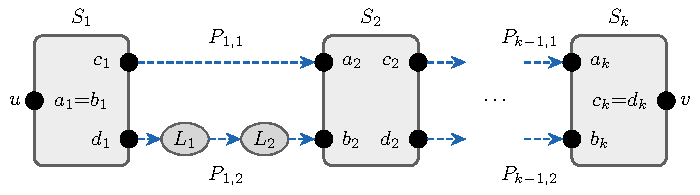
\includegraphics{square-decomposition.pdf}
    \caption{The square decomposition: squares (boxes), links (ellipses) and the directed edges of $F$}
    \label{fig:square-decomposition}
\end{figure}

\begin{example}
\label{ex:decomposition}
In the graph $G_a$ of \cref{ex:counterexamples}, let $p_1 = u, a, t, v$ and $p_2 = u, s, b, v$.
The minimum $u$--$v$ cuts are $\{ua, us\}$, $\{ua, sb\}$, $\{at, bv\}$ and $\{tv, bv\}$, so $F$ contains all edges except $ab$.
The squares are $S_1 = \{u\}$, $S_2 = \{a, b\}$ and $S_3 = \{v\}$, and the links are $\{s\}$ and $\{t\}$ (\cref{fig:decomposition-example}).
The terminals of $S_2$ are $a_2 = c_2 = a$ and $b_2 = d_2 = b$.
The general paths are $P_{1,1} = ua$, $P_{1,2} = us, \{s\}, sb$, $P_{2,1} = at, \{t\}, tv$ and $P_{2,2} = bv$.
\end{example}

\begin{figure}[tb]
    \centering
    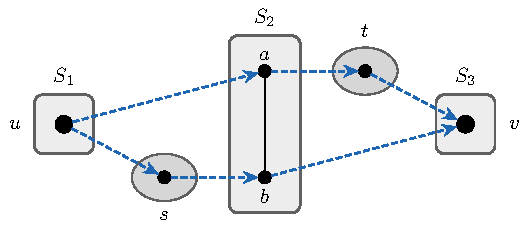
\includegraphics{decomposition-example.pdf}
    \caption{The square decomposition of $G_a$ with respect to $u$ and $v$}
    \label{fig:decomposition-example}
\end{figure}

\begin{example}
\label{ex:worked}
Let $G_1$ be the graph with the vertices $u, v, 1, \dots, 8$ and the edges
\[
u1,\ u2,\ 12,\ 13,\ 23,\ 36,\ 24,\ 45,\ 57,\ 67,\ 68,\ 7v,\ 8v
\]
(\cref{fig:worked-example}).
We have $c(u, v) = 2$ and $d(u, v) = 5$, and we take $p_1 = u, 1, 3, 6, 8, v$ and $p_2 = u, 2, 4, 5, 7, v$.
The minimum $u$--$v$ cuts are $\{u1, u2\}$, $\{36, 24\}$, $\{36, 45\}$, $\{36, 57\}$, $\{68, 7v\}$ and $\{8v, 7v\}$, so $F$ contains all edges except $12$, $13$, $23$ and $67$.
The squares are $S_1 = \{u\}$, $S_2 = \{1, 2, 3\}$, $S_3 = \{6, 7\}$ and $S_4 = \{v\}$, and the links are $\{4\}$, $\{5\}$ and $\{8\}$.
The terminals are $a_2 = 1$, $b_2 = d_2 = 2$, $c_2 = 3$, $a_3 = c_3 = 6$ and $b_3 = d_3 = 7$.
The general paths $P_{1,1}$, $P_{1,2}$, $P_{2,1}$ and $P_{3,2}$ are the single edges $u1$, $u2$, $36$ and $7v$, while $P_{2,2} = 24, \{4\}, 45, \{5\}, 57$ and $P_{3,1} = 68, \{8\}, 8v$.
Every vertex outside $S_2 \cup S_3$ has degree two, two vertices of the same square are adjacent, and the cut $\{36, 24\}$ separates $S_2$ from $S_3$.
Hence $G_1 \in \DC$.
\end{example}

\begin{figure}[tb]
    \centering
    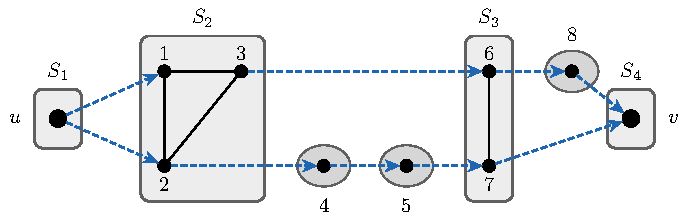
\includegraphics{worked-example.pdf}
    \caption{The graph $G_1$ of \cref{ex:worked} and its square decomposition}
    \label{fig:worked-example}
\end{figure}

\subsection{Separating Shortest Paths}
\label{sec:separating}

By \cref{lem:basic-bounds} and \cref{prop:easy-pairs}(iii), a pair with $c(u, v) = 2$ satisfies $\cp(u, v) = d(u, v)$ if $G$ contains a separating shortest $u$--$v$ path, and $\cp(u, v) = d(u, v) + 1$ otherwise.
Whether a $u$--$v$ path separates $u$ from $v$ is decided inside the squares.

Let $R$ be a $u$--$v$ path.
By \cref{thm:structure}(ii) and \cref{lem:pieces}(iii), the path $R$ contains exactly one of the two edges that enter $S_i$, for $2 \leq i \leq k$, and exactly one of the two edges that leave $S_i$, for $1 \leq i < k$.
Let $x_i$ be the head of the edge of $R$ that enters $S_i$, and let $\alpha_i$ be the head of the other edge that enters $S_i$.
Let $y_i$ be the tail of the edge of $R$ that leaves $S_i$, and let $\beta_i$ be the tail of the other edge that leaves $S_i$.
We put $x_1 = \alpha_1 = u$ and $y_k = \beta_k = v$.
Then $(x_i, \alpha_i)$ is $(a_i, b_i)$ or $(b_i, a_i)$, the pair $(y_i, \beta_i)$ is $(c_i, d_i)$ or $(d_i, c_i)$, and the trace of $R$ in $S_i$ is an $x_i$--$y_i$ path (\cref{fig:square-terminals}).

\begin{figure}[tb]
    \centering
    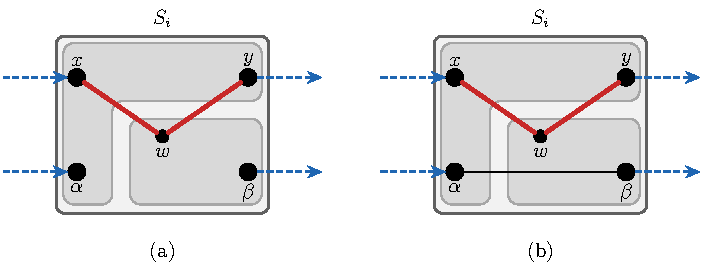
\includegraphics{square-terminals.pdf}
    \caption{A square $S_i$ and a trace $x, w, y$ that separates $\alpha$ from $\beta$ in (a) and does not in (b)}
    \label{fig:square-terminals}
\end{figure}

\begin{lemma}[Separation criterion]
\label{lem:criterion}
Let $c(u, v) = 2$, and let $R$ be a $u$--$v$ path.
The graph $G \setminus R$ contains a $u$--$v$ path if and only if, for every $i \in \{1, \dots, k\}$, the vertices $\alpha_i$ and $\beta_i$ lie in the same component of $S_i \setminus R$.
\end{lemma}

\begin{proof}
Let $1 \leq i < k$.
By \cref{thm:structure}(iv), $R$ contains the edges of one of the general paths from $S_i$ to $S_{i+1}$, and it contains no edge and visits no link of the other one, which we denote by $e_0, L_1, e_1, \dots, L_r, e_r$.
The edge $e_0$ is the edge that leaves $S_i$ and does not lie on $R$, so its tail is $\beta_i$, and likewise the head of $e_r$ is $\alpha_{i+1}$.
The links $L_1, \dots, L_r$ are connected and contain no edge of $R$.
Hence $\beta_i$ and $\alpha_{i+1}$ lie in the same component of $G \setminus R$.

Suppose that $\alpha_i$ and $\beta_i$ lie in the same component of $S_i \setminus R$ for every $i$.
Then $u = \alpha_1$, $\beta_1$, $\alpha_2$, $\beta_2$, \dots, $\alpha_k$, $\beta_k = v$ all lie in the same component of $G \setminus R$.

Conversely, let $Q$ be a $u$--$v$ path of $G \setminus R$, and let $1 \leq i \leq k$.
By \cref{thm:structure}(ii), $Q$ visits $S_i$.
If $i \geq 2$, the path $Q$ contains an edge that enters $S_i$ and does not lie on $R$, so the first vertex of $Q$ in $S_i$ is $\alpha_i$.
If $i = 1$, this vertex is $u = \alpha_1$.
In the same way, the last vertex of $Q$ in $S_i$ is $\beta_i$.
The trace of $Q$ in $S_i$ is therefore an $\alpha_i$--$\beta_i$ path of $S_i \setminus R$.
\end{proof}

\begin{theorem}[Separating shortest paths]
\label{thm:characterization}
Let $G$ be a connected graph, let $u$ and $v$ be two vertices of $G$ with $c(u, v) = 2$, and let $S_1, \dots, S_k$ be the squares of $G$ with respect to $u$ and $v$, with the terminals $a_i, b_i, c_i, d_i$.
Then $\cp(u, v) = d(u, v)$ if and only if there are an index $i$, a pair $(x, \alpha) \in \{(a_i, b_i), (b_i, a_i)\}$, a pair $(y, \beta) \in \{(c_i, d_i), (d_i, c_i)\}$ and an $x$--$y$ path $p$ of $S_i$ such that
(i) $d(u, x) + |p| + d(y, v) = d(u, v)$ and
(ii) the vertices $\alpha$ and $\beta$ lie in different components of $S_i \setminus p$.
Otherwise $\cp(u, v) = d(u, v) + 1$.
\end{theorem}

\begin{proof}
Suppose that $i$, $(x, \alpha)$, $(y, \beta)$ and $p$ satisfy (i) and (ii).
Let $R_x$ be a shortest $u$--$x$ path and let $R_y$ be a shortest $y$--$v$ path of $G$.
By (i), the paths $R_x$, $p$ and $R_y$ form a walk from $u$ to $v$ with $d(u, v)$ edges.
Such a walk repeats no vertex, so it is a shortest $u$--$v$ path $R$.
Let $x_i, \alpha_i, y_i, \beta_i$ be defined for $R$ as above, and let $p'$ be the trace of $R$ in $S_i$, which contains $p$.
We show that $\alpha_i$ and $\alpha$ lie in the same component of $S_i \setminus p$.
This holds if $\alpha_i = \alpha$, in particular if $i = 1$.
Otherwise $(x_i, \alpha_i) = (\alpha, x)$, and the part of $p'$ from $x_i = \alpha$ to $x$ is a path of $S_i$ that shares no edge with $p$ and joins $\alpha$ to $\alpha_i = x$.
In the same way, $\beta_i$ and $\beta$ lie in the same component of $S_i \setminus p$.
By (ii), the vertices $\alpha_i$ and $\beta_i$ lie in different components of $S_i \setminus p$, and hence of its subgraph $S_i \setminus R$.
By \cref{lem:criterion}, $R$ is a separating shortest $u$--$v$ path, and $\cp(u, v) = d(u, v)$ by \cref{lem:basic-bounds}.

Conversely, suppose that $\cp(u, v) = d(u, v)$.
By \cref{lem:basic-bounds}, $G$ contains a separating shortest $u$--$v$ path $R$, and by \cref{lem:criterion}, the vertices $\alpha_i$ and $\beta_i$ lie in different components of $S_i \setminus R$ for some $i$.
Let $p$ be the trace of $R$ in $S_i$, and let $(x, \alpha) = (x_i, \alpha_i)$ and $(y, \beta) = (y_i, \beta_i)$.
Condition (ii) holds because $S_i \setminus R = S_i \setminus p$.
Condition (i) holds because the parts of the shortest path $R$ from $u$ to $x$ and from $y$ to $v$ are shortest paths.

The last statement follows from \cref{prop:easy-pairs}(iii).
\end{proof}

A path $p$ with (i) is a shortest $x$--$y$ path of $G$, because $d(u, v) \leq d(u, x) + d(x, y) + d(y, v)$.
A path $p$ with (ii) has at least one edge, because $S_i$ is connected.
The first part of the proof constructs a separating shortest $u$--$v$ path from $p$.

\begin{example}
\label{ex:criterion}
In the graph $G_a$ (\cref{ex:decomposition}), take $i = 2$, $(x, \alpha) = (a, b)$, $(y, \beta) = (b, a)$ and $p = a, b$.
Then $d(u, a) + |p| + d(b, v) = 3 = d(u, v)$, and the graph $S_2 \setminus p$ has no edge, so it separates $\alpha = b$ from $\beta = a$.
Hence $\cp(u, v) = 3$.

In the graph $G_1$ (\cref{ex:worked}), take $i = 3$, $(x, \alpha) = (6, 7)$, $(y, \beta) = (7, 6)$ and $p = 6, 7$.
Then $d(u, 6) + |p| + d(7, v) = 3 + 1 + 1 = d(u, v)$, and $S_3 \setminus p$ has no edge.
Hence $\cp(u, v) = 5$, and $u, 1, 3, 6, 7, v$ is a minimum cut-path.

Let $G_1'$ be obtained from $G_1$ by adding a vertex $9$ adjacent to $6$ and $7$.
The set $F$, the distances from $u$ and to $v$ and the squares $S_1, S_2, S_4$ do not change, and $S_3 = \{6, 7, 9\}$.
The only paths with at least one edge that satisfy (i) are the edges $13$ and $23$ of $S_2$ and the edge $67$ of $S_3$, and each of the graphs $S_2 \setminus \{13\}$, $S_2 \setminus \{23\}$ and $S_3 \setminus \{67\}$ is connected.
Hence $\cp(u, v) = 6$ in $G_1'$.

Let $G_1''$ be obtained from $G_1$ by removing the vertex $5$ and adding the edge $47$.
Then $d(u, v) = 4$, the squares are those of $G_1$, and no path of a square with at least one edge satisfies (i).
Hence $\cp(u, v) = 5$ in $G_1''$.
\end{example}

\subsection{A Linear-Time Algorithm}
\label{sec:algorithm}

In a graph of $\DC$, the paths $p$ of \cref{thm:characterization} have at most two edges, and a constant number of them has to be tested in each square.

\begin{corollary}
\label{cor:two-edges}
Let $G \in \DC$ and let $u, v$ be two vertices of $G$ with $c(u, v) = 2$.
Then every shortest $u$--$v$ path has at most two edges in every square.
Every path $p$ that satisfies condition (i) of \cref{thm:characterization} has $|p| = d(x, y) \leq 2$.
\end{corollary}

\begin{proof}
Let $x$ be an entering terminal and let $y$ be a leaving terminal of a square $S_i$.
If $x \neq y$, then $c(x, y) \geq 3$ by \cref{thm:structure}(v), and $d(x, y) \leq 2$ by \cref{def:class}.
Hence $d(x, y) \leq 2$ in all cases.
The trace of a shortest $u$--$v$ path in $S_i$ is a shortest path of $G$ from an entering terminal to a leaving terminal of $S_i$.
It contains all edges of the path in $S_i$, because an edge of a path joins two consecutive vertices of the path.
A path $p$ with (i) is a shortest $x$--$y$ path of $G$.
\end{proof}

The set $F$ is computed from $p_1$ and $p_2$.
Let $D$ be the directed graph with the vertex set $V$ that contains, for every edge $xy$ of $G$ outside $p_1 \cup p_2$, the arcs from $x$ to $y$ and from $y$ to $x$, and for every edge $xy$ that $p_1$ or $p_2$ traverses from $x$ to $y$, the arc from $y$ to $x$.
It is the residual graph of the flow that sends one unit along $p_1$ and one along $p_2$.
For a directed network, statement (i) of the following lemma is the theorem of Picard and Queyranne~\cite{PicardQueyranne1980} on the closed sets of the residual graph of a maximum flow, and statement (ii) is their criterion for saturated arcs.
We give the short proofs for the flow of value two in the undirected graph $G$, where every edge outside $p_1 \cup p_2$ has both arcs in $D$.

\begin{lemma}
\label{lem:residual}
Let $c(u, v) = 2$.
(i) For a set $A \subseteq V$ with $u \in A$ and $v \notin A$, the set $\delta(A)$ is a minimum $u$--$v$ cut if and only if no arc of $D$ leads from $A$ to $V \setminus A$.
(ii) An edge $xy$ that $p_1$ or $p_2$ traverses from $x$ to $y$ belongs to $F$ if and only if $x$ and $y$ lie in different strong components of $D$.
\end{lemma}

\begin{proof}
(i) Let $\delta(A)$ be a minimum $u$--$v$ cut.
By \cref{lem:orientation}, it consists of an edge of $p_1$ and an edge of $p_2$, and each of them is traversed by its path from $A$ to $V \setminus A$.
The arcs of these two edges lead into $A$, and no other arc has its ends on different sides.
Conversely, suppose that no arc of $D$ leads from $A$ to $V \setminus A$.
Then every edge of $\delta(A)$ lies on $p_1$ or $p_2$ and is traversed by its path from $A$ to $V \setminus A$.
A path that starts in $A$ and has left $A$ cannot leave $A$ again without returning to $A$ first, so each of $p_1$ and $p_2$ contains exactly one edge of $\delta(A)$.
Hence $\delta(A)$ is a $u$--$v$ cut with two edges.

(ii) Let $p_j$ be the path that contains $xy$.
If $xy \in F$, it lies in a minimum $u$--$v$ cut $\delta(A)$, and $x \in A$, $y \notin A$ by \cref{lem:orientation}(ii).
By (i), no directed path of $D$ leads from $x$ to $y$, so $x$ and $y$ lie in different strong components.
Conversely, suppose that $x$ and $y$ lie in different strong components.
Since $D$ contains the arc from $y$ to $x$, no directed path of $D$ leads from $x$ to $y$.
Let $A$ be the set of all vertices that can be reached from $x$ by directed paths of $D$.
Then $x \in A$, $y \notin A$, and no arc leads from $A$ to $V \setminus A$.
The arcs of the edges of $p_j$ form a directed path from $v$ through $y$ and $x$ to $u$.
Hence $u \in A$, and $v \notin A$ because $y$ can be reached from $v$.
By (i), $\delta(A)$ is a minimum $u$--$v$ cut, and it contains $xy$.
\end{proof}

\begin{algorithm}[tb]
\caption{A minimum cut-path if $c(u, v) = 2$, or two vertices that show $G \notin \DC$}
\label{alg:cut-two}
\begin{algorithmic}[1]
\Require a connected graph $G = (V, E)$ and two vertices $u, v$ with $c(u, v) = 2$
\Ensure $\cp(u, v)$ and a minimum cut-path between $u$ and $v$, or two vertices $x, y$ with $c(x, y) \geq 3$ and $d(x, y) \geq 3$ and a cut-path between $u$ and $v$ with $d(u, v) + 1$ edges
\State compute $d(u, z)$ and $d(z, v)$ for all $z \in V$ by two breadth-first searches \label{line:bfs}
\State compute two edge-disjoint $u$--$v$ paths $p_1$ and $p_2$ \label{line:paths}
\State $F \gets$ the edges of $p_1 \cup p_2$ whose ends lie in different strong components of $D$ \label{line:residual}
\State compute the pieces, the squares $S_1, \dots, S_k$ and their terminals \label{line:pieces}
\For{$i \gets 1$ to $k$} \label{line:loop}
    \For{each $(x, \alpha) \in \{(a_i, b_i), (b_i, a_i)\}$ and $(y, \beta) \in \{(c_i, d_i), (d_i, c_i)\}$ with $x \neq y$ and $\alpha \neq \beta$}
        \State $\ell \gets d(u, v) - d(u, x) - d(y, v)$ \label{line:length}
        \If{$\ell \geq 3$}
            \State record the pair $x, y$ \Comment{$c(x, y) \geq 3$ and $d(x, y) \geq 3$} \label{line:record}
        \EndIf
        \State $\mathcal{P} \gets \emptyset$
        \If{$\ell = 1$ and $xy \in E$}
            \State $\mathcal{P} \gets$ the set that contains the path $x, y$ \label{line:edge}
        \ElsIf{$\ell = 2$}
            \State $q \gets$ an $\alpha$--$\beta$ path of $S_i$ \label{line:q}
            \State $\mathcal{P} \gets$ the set of the paths $x, w, y$ of $S_i$ such that $xw$ or $wy$ is an edge of $q$ \label{line:candidates}
        \EndIf
        \For{each $p \in \mathcal{P}$}
            \If{$\alpha$ and $\beta$ lie in different components of $S_i \setminus p$} \label{line:test}
                \State \Return $d(u, v)$ and $R_x \cup p \cup R_y$ for a shortest $u$--$x$ path $R_x$ and a shortest $y$--$v$ path $R_y$ \label{line:found}
            \EndIf
        \EndFor
    \EndFor
\EndFor
\State $R \gets$ a shortest $u$--$v$ path, $C \gets$ the set of the two edges that leave $S_1$ \label{line:union}
\If{a pair $x, y$ is recorded}
    \State \Return $x, y$ and $R \cup C$ \label{line:certificate}
\EndIf
\State \Return $d(u, v) + 1$ and $R \cup C$ \label{line:not-found}
\end{algorithmic}
\end{algorithm}

\Cref{alg:cut-two} computes the square decomposition and searches every square for a path $p$ as in \cref{thm:characterization} with at most two edges.
For a path with two edges it uses that a path which separates $\alpha$ from $\beta$ shares an edge with every $\alpha$--$\beta$ path of the square.
The algorithm does not test whether $G \in \DC$.

\begin{theorem}
\label{thm:linear-time}
There is an algorithm that, given a connected graph $G = (V, E)$ and two distinct vertices $u, v$ of $G$, decides in $O(|V| + |E|)$ time whether $c(u, v) \leq 2$.
If so, it returns within the same time $\cp(u, v)$ and a minimum cut-path between $u$ and $v$, or it returns two vertices $x, y$ with $c(x, y) \geq 3$ and $d(x, y) \geq 3$, which show that $G \notin \DC$, and a cut-path between $u$ and $v$ with $d(u, v) + 1 \leq \cp(u, v) + 1$ edges.
The second outcome does not occur for $G \in \DC$.
\end{theorem}

\begin{proof}
The algorithm first computes, by at most three augmentations of the algorithm of Ford and Fulkerson~\cite[Section~10.4]{Erickson2019Algorithms}, a flow from $u$ to $v$ of value at most three in which every edge of $G$ carries at most one unit.
Each augmentation is a search in the residual graph of the current flow and takes $O(|V| + |E|)$ time.
The first augmentation succeeds because $G$ is connected.
The cut-value $c(u, v)$ is one if the second augmentation fails, two if the third one fails, and at least three otherwise.
If $c(u, v) = 1$, the algorithm returns $d(u, v)$ and a shortest $u$--$v$ path, which is correct by \cref{prop:easy-pairs}(ii).

Let $c(u, v) = 2$.
The two augmenting paths need not be edge-disjoint, because the second one can traverse an edge of the first one backwards, which cancels the flow on this edge.
The paths $p_1$ and $p_2$ are therefore read from the flow of value two.
Let $H$ be the directed graph formed by the edges that carry flow, each directed along the flow.
In $H$, the vertex $u$ has two more leaving than entering arcs, the vertex $v$ has two more entering than leaving arcs, and every other vertex has as many entering as leaving arcs.
No arc of $H$ leaves the set $X$ of the vertices that can be reached from $u$, so the vertices of $X$ have in total at most as many leaving as entering arcs, and hence $v \in X$.
A search in $H$ therefore finds a $u$--$v$ path $p_1$.
After the removal of the arcs of $p_1$, the same argument with one in place of two gives a $u$--$v$ path $p_2$.
The paths $p_1$ and $p_2$ are edge-disjoint paths of $G$, and the arcs of $H$ that remain form cycles and are not used.
Line~\ref{line:paths} of \cref{alg:cut-two} takes these two paths, and the algorithm runs \cref{alg:cut-two}.

\emph{Correctness.}
By \cref{lem:residual}(ii), line~\ref{line:residual} computes the set $F$, and the direction in which $p_1$ or $p_2$ traverses an edge of $F$ gives its tail and its head.
Line~\ref{line:pieces} therefore computes the squares and the terminals of \cref{def:pieces,def:decomposition}.
Every path $p$ that is tested in line~\ref{line:test} is an $x$--$y$ path of $S_i$ with $\ell$ edges, so it satisfies condition (i) of \cref{thm:characterization}.
If the test succeeds, $p$ also satisfies condition (ii).
By the proof of \cref{thm:characterization}, the set returned in line~\ref{line:found} is then a separating shortest $u$--$v$ path, which is a cut-path with $d(u, v) = \cp(u, v)$ edges.
A path returned in line~\ref{line:found} is thus a minimum cut-path in every connected graph.

If line~\ref{line:length} gives $\ell \geq 3$ for two terminals $x \neq y$, then $d(x, y) \geq \ell \geq 3$, because $d(u, v) \leq d(u, x) + d(x, y) + d(y, v)$, and $c(x, y) \geq 3$ by \cref{thm:structure}(v).
A pair recorded in line~\ref{line:record} therefore shows that $G \notin \DC$, and no pair is recorded if $G \in \DC$.

Suppose now that $\cp(u, v) = d(u, v)$ and that no pair is recorded.
By \cref{thm:characterization}, there are $i$, $(x, \alpha)$, $(y, \beta)$ and $p$ with (i) and (ii).
Then $\alpha \neq \beta$ and the path $p$ has at least one edge, so $x \neq y$, and line~\ref{line:length} gives $\ell = |p|$ for these terminals.
Since the pair $x, y$ is not recorded, $\ell \in \{1, 2\}$.
If $\ell = 1$, then $p$ is the path of line~\ref{line:edge}.
If $\ell = 2$, let $p = x, w, y$.
The path $q$ of line~\ref{line:q} is not a path of $S_i \setminus p$, so it contains the edge $xw$ or the edge $wy$.
In both cases $p \in \mathcal{P}$, so the algorithm returns in line~\ref{line:found}, for this path or for an earlier one.

Hence, if the algorithm reaches line~\ref{line:not-found}, then $\cp(u, v) = d(u, v) + 1$.
The set $C$ of line~\ref{line:union} is a minimum $u$--$v$ cut by \cref{thm:structure}(i), and $R$ contains exactly one of its edges by \cref{lem:orientation}(ii).
Hence $R \cup C$ is a cut-path with $d(u, v) + 1$ edges, which is a minimum cut-path in line~\ref{line:not-found} and has at most $\cp(u, v) + 1$ edges in line~\ref{line:certificate}.

\emph{Running time.}
The graph is given by adjacency lists.
Breadth-first search~\cite[Section~8.4]{Erickson2019Algorithms} and the computation of strong components~\cite{Tarjan1972DFS} take $O(|V| + |E|)$ time.
The paths $p_1$ and $p_2$ are found by two searches in $H$.
Lines~\ref{line:bfs} to~\ref{line:pieces} consist of a constant number of such computations and of one search in $G \setminus F$ for the pieces.
Let $S_i$ have $n_i$ vertices and $m_i$ edges.
For each of the at most four choices of $(x, \alpha)$ and $(y, \beta)$, the path $q$ is found by one search in $S_i$.
The path $q$ has at most two edges at $x$ and at most two edges at $y$, so $\mathcal{P}$ has at most four members.
Whether $x, w, y$ is a path of $S_i$ is decided for each of these vertices $w$ after marking the neighbors of $x$ and of $y$.
A vertex of $S_i$ is an end of at most four edges outside $S_i$, the edges that enter or leave $S_i$, so its neighbors are marked in $O(m_i + 1)$ time.
The test of line~\ref{line:test} is one search in $S_i \setminus p$.
The square $S_i$ therefore takes $O(n_i + m_i)$ time.
The squares are pairwise disjoint, so the loop of line~\ref{line:loop} takes $O(|V| + |E|)$ time.
The paths $R_x$, $R_y$ and $R$ are read from the breadth-first search trees.
\end{proof}

\Cref{alg:cut-two} returns $\cp(u, v)$ and a minimum cut-path whenever no pair is recorded, in particular if every entering terminal of every square is at distance at most two from every leaving terminal of the same square.

\begin{example}
\label{ex:two-edges}
Let $G_a^{+}$ be obtained from the graph $G_a$ of \cref{ex:counterexamples} by adding a vertex $r$ adjacent to $u$ and $b$.
The vertices of degree greater than two are $u$, $a$ and $b$, which are pairwise at distance at most two, so $G_a^{+} \in \DC$.
The minimum $u$--$v$ cuts are $\{at, bv\}$ and $\{tv, bv\}$.
Hence the squares are $S_1 = \{u, s, r, a, b\}$ and $S_2 = \{v\}$, the only link is $\{t\}$, and $c_1 = a$ and $d_1 = b$ for $p_1 = u, a, t, v$.
For $(x, \alpha) = (u, u)$ and $(y, \beta) = (b, a)$, \cref{alg:cut-two} computes $\ell = 3 - 0 - 1 = 2$.
Let $q$ be the path $u, a$.
Its only edge is $ua$, so $w = a$, and $\mathcal{P}$ contains the path $p = u, a, b$.
The vertex $a$ is isolated in $S_1 \setminus p$, so the algorithm returns $3$ and the path $u, a, b, v$.
\end{example}

\begin{corollary}
\label{cor:class-pairs}
Let $G \in \DC$ and let $u, v$ be two distinct vertices of $G$.
If $c(u, v) \leq 2$, in particular if $d(u, v) \geq 3$, then $\cp(u, v)$ and a minimum cut-path between $u$ and $v$ are computed in $O(|V| + |E|)$ time.
If $d(u, v) = 1$, they are computed by one computation of a minimum $u$--$v$ cut.
\end{corollary}

\begin{proof}
A pair with $d(u, v) \geq 3$ has $c(u, v) \leq 2$ by \cref{def:class}.
The first statement is \cref{thm:linear-time}, whose second outcome does not occur for $G \in \DC$, and the second is \cref{prop:easy-pairs}(i).
A minimum $u$--$v$ cut is computed in polynomial time by a maximum flow~\cite[Sections~10.3 and~10.4]{Erickson2019Algorithms}.
\end{proof}

\section{From Pairs at Distance Two to a Zigzag Problem}
\label{sec:zz-zigzag}

An \emph{instance of the open case} is a triple $(G, u, v)$ with $G \in \DC$ and vertices $u, v$ of $G$ with $d(u, v) = 2$ and $c(u, v) \geq 3$.
By \cref{prop:easy-pairs}(iv), we have $\cp(u, v) \in \{c(u, v), c(u, v) + 1\}$, so the question is whether $\cp(u, v) = c(u, v)$.
\Cref{thm:zz-reduction} maps such an instance to an instance of a problem on a preordered set with the same answer, and \cref{lem:zz-valid} turns that problem into the search for a walk.

\subsection{Preorders and the Problem ZZ}
\label{sec:zz-preorders}

\begin{definition}[Preorders]
\label{def:zz-preorder}
A \emph{preorder} $\leq$ on a finite set is a reflexive and transitive relation.
We write $x < y$ if $x \leq y$ and not $y \leq x$.
We write $x \sim y$, and call $x$ and $y$ \emph{tied}, if $x \leq y$ and $y \leq x$, and $[x]$ is the class of $x$ under this equivalence relation.
We write $x \parallel y$, and call $x$ and $y$ \emph{incomparable}, if neither $x \leq y$ nor $y \leq x$.
For a set $S$, we put $\dn S = \{x : x \leq y \text{ for some } y \in S\}$, $\upp S = \{x : x \geq y \text{ for some } y \in S\}$, $\dn x = \dn \{x\}$ and $\upp x = \upp \{x\}$.
A \emph{down-set} $D$ satisfies $\dn D = D$, and an \emph{up-set} $D$ satisfies $\upp D = D$.
Complements of down-sets are up-sets, intersections and unions of down-sets are down-sets, $\dn S$ is a down-set, and the complement of $\upp S$ is a down-set.
If $x \leq y < z$ or $x < y \leq z$, then $x < z$.
\end{definition}

\begin{definition}[ZZ and P2]
\label{def:zz-zz}
An instance of \emph{ZZ} is a tuple $(Q, \leq, R, u, v)$ that consists of a finite set $Q$ with a preorder $\leq$ such that $u \leq x \leq v$ for every $x \in Q$ and $u < v$, and a set $R$ of pairs $\{a, b\} \subseteq Q$ with $a < b$.
The pairs of $R$ are its \emph{edges}.
We write $ab$ for an edge with $a < b$, and we call $a$ its \emph{lower end} and $b$ its \emph{upper end}.
For a down-set $D$ of $Q$ with $u \in D$ and $v \notin D$, the graph $G_D$ on $Q$ has as its edges the edges of $R$ with exactly one end in $D$.
The instance is a \emph{yes-instance} if $u$ and $v$ are connected in $G_D$ for some such $D$.
Two elements $x$ and $y$ \emph{meet below} if some element $z$ satisfies $zx \in R$ and $zy \in R$, and they \emph{meet above} if some element $z$ satisfies $xz \in R$ and $yz \in R$.
The instance satisfies \emph{P2} if every two incomparable elements meet below or meet above.
\end{definition}

A path of $G_D$ alternates between $D$ and $Q \setminus D$, which gives ZZ its name (zigzag).

\begin{definition}[Valid walks]
\label{def:zz-valid}
Let $(Q, \leq, R, u, v)$ be an instance of ZZ.
A \emph{walk} is a sequence $P = x_0, \dots, x_q$ of elements with the ends $u$ and $v$, in either order, whose positions $0, \dots, q$ are labeled alternately \emph{low} and \emph{high}.
The end $u$ is low, the end $v$ is high, and for every $i < q$, the pair of $x_i$ and $x_{i+1}$ is an edge of $R$ whose lower end is at the low position.
Elements may repeat.
The elements at low positions are the \emph{lows} of $P$, the elements at high positions are its \emph{highs}, and $q$ is its \emph{length}.
The walk is \emph{valid} if no high is $\leq$ a low.
For a valid walk, we put $U_P = \upp \{\text{highs of } P\}$ and $L_P = \dn \{\text{lows of } P\}$.
A valid walk is \emph{shortest} if no valid walk has a smaller length.
\end{definition}

The reversal $x_q, \dots, x_0$ of a valid walk, with the same labels, is a valid walk of the same length.
\Cref{fig:zz-walk}(b) shows a valid walk.

\begin{figure}[tb]
    \centering
    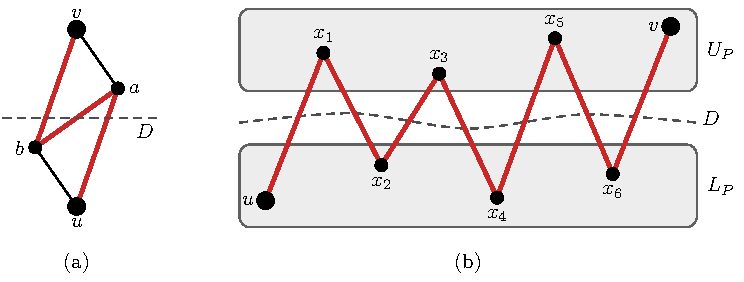
\includegraphics{zz-walk.pdf}
    \caption{(a) The ZZ instance of $G_b$ and the walk $u, a, b, v$ (\cref{ex:zz-instance}); (b) a valid walk and a down-set $D$ between $L_P$ and $Q \setminus U_P$; larger elements lie higher}
    \label{fig:zz-walk}
\end{figure}

\begin{lemma}[Valid walks and yes-instances]
\label{lem:zz-valid}
Let $(Q, \leq, R, u, v)$ be an instance of ZZ.
(a) If $P$ is a valid walk, then $U_P \cap L_P = \emptyset$, and every down-set $D$ with $L_P \subseteq D \subseteq Q \setminus U_P$ satisfies $u \in D$ and $v \notin D$, and $u$ and $v$ are connected in $G_D$.
(b) If $u$ and $v$ are connected in $G_D$ for a down-set $D$ with $u \in D$ and $v \notin D$, then a valid walk exists.
(c) The instance is a yes-instance if and only if a valid walk exists.
(d) The elements at distinct positions of a shortest valid walk are distinct.
\end{lemma}

\begin{proof}
(a) An element of $U_P \cap L_P$ would give $h \leq x \leq \ell$ for a high $h$ and a low $\ell$, against validity.
Let $D$ be as stated.
The element $u$ is a low and $v$ is a high, so $u \in D$ and $v \notin D$.
Every edge of $P$ has its lower end at a low position, hence in $D$, and its upper end at a high position, hence outside $D$.
So $P$ is a walk of $G_D$ between $u$ and $v$.

(b) Take a $u$--$v$ path of $G_D$.
An edge $ab$ of $G_D$ has exactly one end in $D$, and since $a < b$ and $D$ is a down-set, this end is $a$.
So the vertices of the path alternate between $D$ and $Q \setminus D$.
Label those in $D$ low and the others high, which gives a walk.
If a high $h$ were $\leq$ a low $\ell$, then $\ell \in D$ would give $h \in D$, so the walk is valid.

(c) This follows from (b) and from (a) with $D = L_P$.

(d) Let $x_i = x_j$ with $i < j$.
By validity, no element is both a high and a low, so the positions $i$ and $j$ have the same label.
Removing $x_{i+1}, \dots, x_j$ leaves a valid walk of smaller length.
\end{proof}

\subsection{Reduction of the Open Case to ZZ with P2}
\label{sec:zz-reduction}

Throughout this subsection, $(G, u, v)$ is an instance of the open case with $n$ vertices, and $c = c(u, v)$.
A \emph{minimum side} is a set $A \subseteq V$ with $u \in A$, $v \notin A$ and $|\delta(A)| = c$.
By \cref{lem:minimum-cuts}, the minimum $u$--$v$ cuts are exactly the sets $\delta(A)$ for the minimum sides $A$.

\begin{lemma}[Minimum sides]
\label{lem:zz-sides}
(a) If $A$ and $B$ are minimum sides, then $A \cap B$ and $A \cup B$ are minimum sides, and no edge of $G$ joins $A \setminus B$ and $B \setminus A$.
(b) Let $A$ be a minimum side, let $Y \subseteq V \setminus \{u, v\}$ with $|\delta(Y)| \leq 2$, and let $k$ be the number of edges of $\delta(A)$ with an end in $Y$.
Then $k \leq 1$.
If $k = 1$, then $A \setminus Y$ and $A \cup Y$ are minimum sides.
\end{lemma}

\begin{proof}
(a) The sets $A \cap B$ and $A \cup B$ contain $u$ and not $v$, so each of their boundaries has at least $c$ edges.
By \cref{lem:uncrossing}, the two boundaries have $2c - 2m(A, B)$ edges together, which forces $m(A, B) = 0$ and two minimum sides.

(b) An edge with no end in $Y$ lies in $\delta(A \setminus Y)$ if and only if it lies in $\delta(A)$, and the same holds for $\delta(A \cup Y)$.
An edge with both ends in $Y$ lies in neither set.
An edge of $\delta(Y)$ whose end outside $Y$ is $y$ lies in $\delta(A \setminus Y)$ if $y \in A$ and in $\delta(A \cup Y)$ if $y \notin A$.
Hence $|\delta(A \setminus Y)| + |\delta(A \cup Y)| = 2(c - k) + |\delta(Y)| \leq 2c - 2k + 2$.
The sets $A \setminus Y$ and $A \cup Y$ contain $u$ and not $v$, so the left-hand side is at least $2c$.
This gives $k \leq 1$, and for $k = 1$ it forces $|\delta(A \setminus Y)| = |\delta(A \cup Y)| = c$.
\end{proof}

We put
\[
Q = \{u\} \cup \{x \in V \setminus \{u\} : c(u, x) \geq 3\},
\]
so $v \in Q$.

\begin{lemma}[The set $Q$]
\label{lem:zz-q}
(a) Every vertex $x \notin Q$ lies in a set $Y \subseteq V \setminus Q$ with $|\delta(Y)| \leq 2$.
(b) Every two distinct $x, y \in Q$ satisfy $c(x, y) \geq 3$ and $d(x, y) \leq 2$.
(c) If $\delta(A)$ contains a $u$--$v$ path for a minimum side $A$, then all vertices of this path lie in $Q$.
\end{lemma}

\begin{proof}
(a) We have $x \neq u$ and $c(x, u) \leq 2$, so by \cref{lem:minimum-cuts} there is a set $Y$ with $x \in Y$, $u \notin Y$ and $|\delta(Y)| \leq 2$.
A vertex $y \in Y \cap Q$ would satisfy $y \neq u$, and $\delta(Y)$ would be a $u$--$y$ cut with at most two edges.

(b) If $x = u$ or $y = u$, then $c(x, y) \geq 3$ by the definition of $Q$.
Otherwise $c(x, u) \geq 3$ and $c(u, y) \geq 3$ give $c(x, y) \geq 3$ by \cref{prop:class}.
As $G \in \DC$, we have $d(x, y) \leq 2$.

(c) Suppose that the path has a vertex $x \notin Q$, and let $Y$ be the set of (a), which contains neither $u$ nor $v$.
The path enters $Y$ by one edge and leaves it by a later edge, and these are two edges of $\delta(A)$ with an end in $Y$, against \cref{lem:zz-sides}(b).
\end{proof}

\begin{definition}[The ZZ instance of $(G, u, v)$]
\label{def:zz-instance}
For $x, y \in Q$, let $x \leq y$ if every minimum side that contains $y$ contains $x$.
Let $R$ be the set of the edges of $G$ with both ends in $Q$ whose ends are not tied.
The \emph{ZZ instance of} $(G, u, v)$ is $(Q, \leq, R, u, v)$.
\end{definition}

\begin{lemma}[Properties of the ZZ instance]
\label{lem:zz-instance}
(a) The relation $\leq$ is a preorder on $Q$ with $u \leq x \leq v$ for every $x \in Q$, and $u < v$.
Two incomparable elements are not adjacent in $G$, so every edge in $R$ joins two strictly comparable elements, and $(Q, \leq, R, u, v)$ is an instance of ZZ.
(b) For every minimum side $A$, the set $A \cap Q$ is a down-set of $(Q, \leq)$ that contains $u$ and not $v$.
Every such down-set is $A \cap Q$ for some minimum side $A$.
(c) The instance satisfies P2.
\end{lemma}

\begin{proof}
(a) Reflexivity and transitivity follow from the definition.
Every minimum side contains $u$ and none contains $v$, so $u \leq x \leq v$.
A minimum side exists, so $v \leq u$ fails.
If $x \parallel y$, some minimum side $A_1$ contains $x$ and not $y$, and some minimum side $A_2$ contains $y$ and not $x$.
By \cref{lem:zz-sides}(a), no edge joins $x \in A_1 \setminus A_2$ and $y \in A_2 \setminus A_1$.

(b) The first statement follows from the definition of $\leq$.
Let $D$ be a down-set with $u \in D$ and $v \notin D$, and let $y \in D$.
Some minimum side contains $y$, since otherwise $v \leq y$ holds vacuously and $v \in D$.
By \cref{lem:zz-sides}(a), the intersection $S_y$ of all minimum sides that contain $y$ is a minimum side, and by the definition of $\leq$, we have $S_y \cap Q = \dn y \subseteq D$.
Since $u \in D$, the union $A$ of the sets $S_y$ with $y \in D$ is a minimum side by \cref{lem:zz-sides}(a), and $A \cap Q = D$.

(c) Let $x \parallel y$.
By (a), the elements $x$ and $y$ are not adjacent, so by \cref{lem:zz-q}(b), they have a common neighbor $z$ in $G$.
We first show that $z \in Q$.
Suppose not, and let $Y$ be the set of \cref{lem:zz-q}(a) for $z$.
Since $x, y \notin Y$, the edges $xz$ and $yz$ lie in $\delta(Y)$.
Let $A_1$ and $A_2$ be as in the proof of (a).
For $i \in \{1, 2\}$, one of the edges $xz$ and $yz$ lies in $\delta(A_i)$, because $A_i$ contains exactly one of $x$ and $y$.
By \cref{lem:zz-sides}(b), $A_1 \setminus Y$ and $A_2 \cup Y$ are minimum sides.
The edge $xz$ joins $(A_1 \setminus Y) \setminus (A_2 \cup Y)$ and $(A_2 \cup Y) \setminus (A_1 \setminus Y)$, against \cref{lem:zz-sides}(a) (\cref{fig:p2-outside}).

So $z \in Q$, and by (a), $z$ is comparable with $x$ and with $y$.
If $x \leq z \leq y$ or $y \leq z \leq x$, then $x$ and $y$ would be comparable.
If $z \sim x$, then the comparability of $z$ and $y$ would make $x$ and $y$ comparable, so $z$ is not tied with $x$, and likewise not with $y$.
Hence $z < x$ and $z < y$, or $z > x$ and $z > y$, and $xz$ and $yz$ are edges of $R$.
\end{proof}

\begin{figure}[tb]
    \centering
    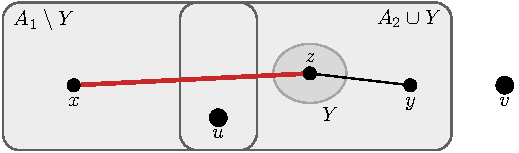
\includegraphics{p2-outside.pdf}
    \caption{The common neighbor $z \notin Q$ in the proof of \cref{lem:zz-instance}(c): the edge $xz$ joins the two differences of two minimum sides}
    \label{fig:p2-outside}
\end{figure}

\begin{theorem}[Reduction]
\label{thm:zz-reduction}
Let $(G, u, v)$ be an instance of the open case with $n$ vertices.
Its ZZ instance $(Q, \leq, R, u, v)$ satisfies P2, has $|Q| \leq n$ and is computable in $O(n^5)$ time.
We have $\cp(u, v) = c(u, v)$ if and only if it is a yes-instance of ZZ.
For a down-set $D$ with $u \in D$ and $v \notin D$ such that $u$ and $v$ are connected in $G_D$, one maximum-flow computation, in $O(n^3)$ time, gives a minimum side $A$ with $A \cap Q = D$, and $\delta(A)$ is a minimum cut-path between $u$ and $v$.
\end{theorem}

\begin{proof}
The first statement on the instance is \cref{lem:zz-instance}(c), and $Q \subseteq V$.

\emph{Answer.}
Let $A$ be a minimum side such that $\delta(A)$ contains a $u$--$v$ path $\pi$.
By \cref{lem:zz-q}(c), all vertices of $\pi$ lie in $Q$.
By \cref{lem:zz-instance}(b), $D = A \cap Q$ is a down-set with $u \in D$ and $v \notin D$.
Every edge of $\pi$ has exactly one end in $D$, so its ends are not tied, because a down-set contains the whole class of each of its elements.
So $\pi$ is a path of $G_D$.

Conversely, let $u$ and $v$ be connected in $G_D$, and let $A$ be a minimum side with $A \cap Q = D$, which exists by \cref{lem:zz-instance}(b).
Every edge of a $u$--$v$ path of $G_D$ has both ends in $Q$ and exactly one end in $D$, hence exactly one end in $A$.
So $\delta(A)$ contains this path, and it is a cut-path with $c$ edges, which is a minimum cut-path by \cref{lem:basic-bounds}.
The equivalence is now \cref{prop:open-pairs}.

\emph{Time.}
The set $Q$ takes one test $c(u, x) \geq 3$ per vertex, each by at most three augmenting-path searches, and $c$ takes one maximum-flow computation.
For $x \neq y$, we have $x \leq y$ if $x = u$ or $y = v$.
Otherwise $x \leq y$ holds if and only if no minimum side contains $y$ but not $x$, that is, if and only if the least $|\delta(S)|$ over all sets $S$ with $\{u, y\} \subseteq S \subseteq V \setminus \{x, v\}$ exceeds $c$.
This is one maximum-flow computation between $\{u, y\}$ and $\{x, v\}$.
For a down-set $D$, a set $S$ with $D \subseteq S \subseteq V \setminus (Q \setminus D)$ and least $|\delta(S)|$ is a minimum side with $S \cap Q = D$ by \cref{lem:zz-instance}(b), and it is found by one maximum-flow computation.
We have $c \leq n$, so each of these at most $|Q|^2 + 1$ computations stops after at most $c + 1$ augmenting-path searches and takes $O(n^3)$ time.
\end{proof}

\begin{example}
\label{ex:zz-instance}
In the graph $G_b$ of \cref{ex:counterexamples}, the vertices $s$ and $t$ have degree two, and $u$ is joined to each of $a$, $b$ and $v$ by three edge-disjoint paths, so $c = 3$ and $Q = \{u, a, b, v\}$.
The minimum sides are $\{u\}$, $\{u, s\}$, $\{u, s, b\}$, $\{u, s, b, a\}$ and $\{u, s, b, a, t\}$.
Hence $u < b < a < v$, and $R$ consists of the edges $ua$, $ub$, $ba$, $av$ and $bv$ (\cref{fig:zz-walk}(a)).
The walk $u, a, b, v$ with the lows $u, b$ and the highs $a, v$ is valid, and $D = \{u, b\}$ is a down-set with $L_P \subseteq D \subseteq Q \setminus U_P$.
The minimum side with $A \cap Q = D$ is $A = \{u, s, b\}$, and $\delta(A) = \{ua, ab, bv\}$ is the minimum cut-path of \cref{ex:counterexamples}.
\end{example}

\begin{remark}
\label{rem:zz-no-p2}
The equivalence in \cref{thm:zz-reduction} uses only $c(u, v) \geq 3$, and the hypothesis $G \in \DC$ is used only for P2.
Since $c_0 \geq 4$ in \cref{thm:dt-hardness}, ZZ without P2 is NP-complete.
In the graph $G_\varphi$, P2 fails for a positive and a negative occurrence vertex of two different variables, which are incomparable and have no common neighbor.
\end{remark}

\section{A Polynomial Algorithm for Pairs at Distance Two}
\label{sec:pa-polynomial}

By \cref{lem:zz-valid}, a yes-instance of ZZ has a shortest valid walk, and it suffices to find a down-set between its lows and its highs.
\Cref{thm:pa-formulas} shows that, under P2, a down-set of this kind is described by a formula over at most 28 elements.
Enumerating these formulas gives the algorithm of \cref{thm:pa-open-case}.

Throughout this section, $(Q, \leq, R, u, v)$ is an instance of ZZ with P2.
We write $\MB(x)$ and $\MA(x)$ for the sets of the elements that meet $x$ below and above, respectively.
The \emph{reversed instance} $(Q, \geq, R, v, u)$ has the same pairs in $R$, with lower and upper ends exchanged, and it is an instance of ZZ with P2.
A valid walk of the original instance, with the labels low and high exchanged, is a valid walk of the reversed instance of the same length.
This exchanges $\dn$ and $\upp$, $\MB$ and $\MA$, and $L_P$ and $U_P$, and we call the resulting statements \emph{dual}.

\subsection{Detours}
\label{sec:pa-detours}

Until the end of the proof of \cref{thm:pa-formulas}, $P = x_0, \dots, x_q$ is a shortest valid walk.
By \cref{lem:zz-valid}(d), an element on $P$ has one position, which we denote by $\pos(x)$.
The positions of the highs have one parity and the positions of the lows have the other.
Let $A_P$ be the set of the highs with no high strictly below, and let $B_P$ be the set of the lows with no low strictly above.
The reversed instance exchanges $A_P$ and $B_P$.
For $w \in A_P$, let $\Pos[w]$ be the set of the positions of the highs tied with $w$, and for $w \in B_P$, let $\Pos[w]$ be the set of the positions of the lows tied with $w$.

\begin{lemma}[Basic facts]
\label{lem:pa-basic}
(a) We have $U_P = \upp A_P$ and $L_P = \dn B_P$.
So a down-set contains $L_P$ if and only if it contains $B_P$, and it misses $U_P$ if and only if it misses $A_P$.
(b) A high $e \leq a$ with $a \in A_P$ is tied with $a$ and lies in $A_P$.
A low $f \geq b$ with $b \in B_P$ is tied with $b$ and lies in $B_P$.
\end{lemma}

\begin{proof}
(a) As $Q$ is finite, every high lies above a minimal high, and every low lies below a maximal low.
(b) The relation $e < a$ is excluded by the definition of $A_P$, and a high strictly below $e$ would be strictly below $a$.
The second statement is dual.
\end{proof}

\begin{lemma}[One detour]
\label{lem:pa-one}
(a) Let $x \in Q$, and let $a, a' \in A_P \cap \MB(x)$ with $p = \pos(a) < \pos(a') = p'$.
If no low at a position outside $(p, p')$ is $\geq x$, then $p' - p \leq 4$.
(b) Let $y \in Q$, and let $b, b' \in B_P \cap \MA(y)$ with $p = \pos(b) < \pos(b') = p'$.
If no high at a position outside $(p, p')$ is $\leq y$, then $p' - p \leq 4$.
(c) If $x \notin L_P$, then any two elements of $A_P \cap \MB(x)$ have positions at distance at most four, so $|A_P \cap \MB(x)| \leq 3$.
If $y \notin U_P$, the same holds for $B_P \cap \MA(y)$.
\end{lemma}

\begin{proof}
(a) Let $z$ be a common lower neighbor of $a$ and $x$, and let $z'$ be a common lower neighbor of $a'$ and $x$.
Consider the walk $x_0, \dots, x_p, z, x, z', x_{p'}, \dots, x_q$ of length $p + 4 + q - p'$ (\cref{fig:one-detour}(a)), in which $z$ and $z'$ are low, $x$ is high, and the other elements keep their labels.
It is valid.
Indeed, a kept high $e \leq z$ would give $e < a$ because $z < a$, against $a \in A_P$, and the same holds for $z'$ and $a'$.
Also $x \not\leq z$ and $x \not\leq z'$, because $z, z' < x$, and $x$ is not $\leq$ a kept low by the hypothesis.
As $P$ is shortest, $p + 4 + q - p' \geq q$.

(b) This is the dual of (a).

(c) If $x \notin L_P$, then no low is $\geq x$, so (a) applies.
The positions of the elements of $A_P$ have the same parity, so at most three of them lie at pairwise distance at most four.
The second statement is dual.
\end{proof}

\begin{figure}[tb]
    \centering
    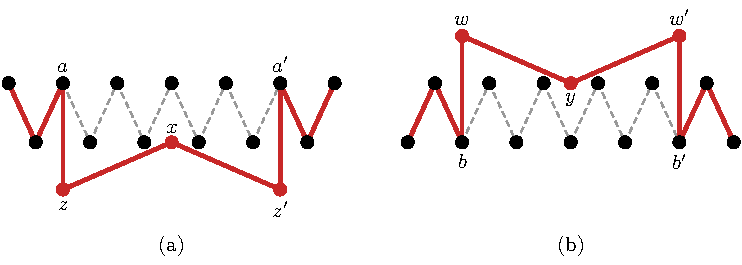
\includegraphics{one-detour.pdf}
    \caption{The walks in the proof of \cref{lem:pa-one}: the red part replaces the gray part of $P$; larger elements lie higher}
    \label{fig:one-detour}
\end{figure}

\begin{lemma}[Two detours]
\label{lem:pa-two}
Let $a \in A_P$ and $h \in B_P$ with $h \not\leq a$, and let $Z = \Pos[a] \cup \Pos[h]$.
Let $p_1 < p_2 < p_3 < p_4$ be positions such that the elements at $p_1$ and at one of $p_2, p_3$ lie in $A_P \cap \MB(h)$, the elements at $p_4$ and at the other of $p_2, p_3$ lie in $B_P \cap \MA(a)$, and $Z \subseteq (p_1, p_2) \cup (p_3, p_4)$.
Then $(p_2 - p_1) + (p_4 - p_3) \leq 8$.
\end{lemma}

\begin{proof}
Let $a_1, a_2 \in A_P \cap \MB(h)$ be the elements at $p_1$ and at the other position, and let $z_i$ be a common lower neighbor of $a_i$ and $h$.
Let $b_1, b_2 \in B_P \cap \MA(a)$ be the elements at the remaining position and at $p_4$, and let $w_i$ be a common upper neighbor of $b_i$ and $a$.
Let $W$ be the sequence $x_{p_2}, \dots, x_{p_3}$ if $a_2$ is at $p_2$, and the sequence $x_{p_3}, \dots, x_{p_2}$ if $a_2$ is at $p_3$.
Consider the walk
\[
x_0, \dots, x_{p_1}, z_1, h, z_2, W, w_1, a, w_2, x_{p_4}, \dots, x_q,
\]
in which $z_1$, $z_2$ and $a$ are low, $h$, $w_1$ and $w_2$ are high, and the other elements, which we call kept, keep their labels (\cref{fig:two-detours}).
Its length is $p_1 + 4 + (p_3 - p_2) + 4 + (q - p_4)$, and no kept element has its position in $Z$.

We show that the walk is valid.
Let $e$ be a kept high and $f$ a kept low.
(1) We have $e \not\leq f$, as $P$ is valid.
(2) If $e \leq a$, then $\pos(e) \in \Pos[a]$ by \cref{lem:pa-basic}(b), which is not kept.
(3) If $e \leq z_i$, then $e < a_i$, against $a_i \in A_P$.
(4) If $h \leq f$, then $\pos(f) \in \Pos[h]$ by \cref{lem:pa-basic}(b), which is not kept.
(5) We have $h \not\leq a$ by hypothesis.
(6) We have $h \not\leq z_i$, because $z_i < h$.
(7) If $w_i \leq f$, then $b_i < f$, against $b_i \in B_P$.
(8) We have $w_i \not\leq a$, because $a < w_i$.
(9) If $w_i \leq z_j$, then $b_i < w_i \leq z_j < h$, so $b_i < h$, and $h$ is a low, against $b_i \in B_P$.

As $P$ is shortest, the length of the walk is at least $q$, which is the claim.
\end{proof}

\begin{figure}[tb]
    \centering
    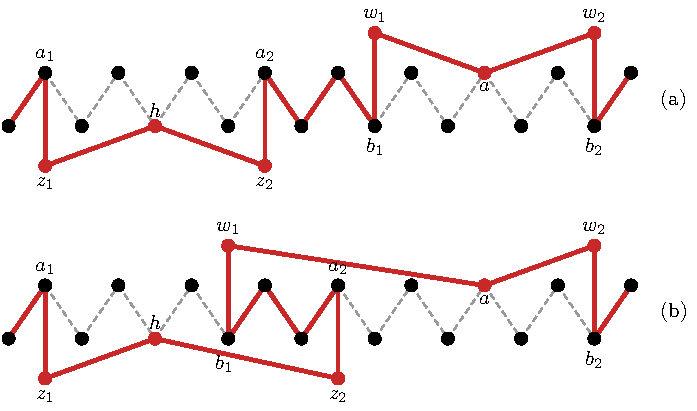
\includegraphics{two-detours.pdf}
    \caption{The walk of \cref{lem:pa-two} for $a_2$ at $p_2$ in (a) and for $a_2$ at $p_3$ in (b); the gray parts of $P$ hold the positions of $Z$}
    \label{fig:two-detours}
\end{figure}

\subsection{Atoms and Formulas}
\label{sec:pa-atoms}

\begin{definition}[Atoms and formulas]
\label{def:pa-atoms}
For elements $x$ and $x'$, the \emph{atoms} are the sets
\begin{align*}
\FR(x, x') &= \dn \bigl(Q \setminus (\MA(x) \cup \MA(x') \cup \upp x \cup \upp x')\bigr),\\
\ER(x, x') &= Q \setminus \upp \bigl(Q \setminus (\MB(x) \cup \MB(x') \cup \dn x \cup \dn x')\bigr),\\
\EP(x) &= Q \setminus \upp \bigl(Q \setminus (\MB(x) \cup (\dn x \setminus [x]))\bigr).
\end{align*}
For elements $x_1, \dots, x_8$ and sets $S, S' \subseteq Q$, an \emph{F-formula} is the set
\[
\FR(x_1, x_2) \cup \FR(x_3, x_4) \cup \FR(x_5, x_6) \cup \dn S \cup \bigl((\EP(x_5) \cup \EP(x_6)) \setminus \upp S'\bigr)
\]
with $|S| \leq 16$ and $|S'| \leq 6$, and an \emph{E-formula} is the set
\[
\bigl(\ER(x_1, x_2) \cap \ER(x_3, x_4) \cap \ER(x_5, x_6) \cap \ER(x_7, x_8)\bigr) \setminus \upp S
\]
with $|S| \leq 16$.
In both, any of the terms with two elements may be omitted, the last term of an F-formula is omitted together with $\FR(x_5, x_6)$, and the empty intersection is $Q$.
\end{definition}

Every atom and every formula is a down-set, because $\dn S$ and the complement of $\upp S$ are down-sets.
An F-formula is built from at most $6 + 16 + 6 = 28$ elements and an E-formula from at most $8 + 16 = 24$ elements.

For $a \in A_P$, we put $C(a) = B_P \cap \MA(a)$ and $\win(a) = A_P \cap \MB(a)$, and for $b \in B_P$, we put $C'(b) = A_P \cap \MB(b)$.
The elements of $C(a)$ and $C'(b)$ are the \emph{contacts} of $a$ and $b$.
Two elements of $A_P$, or two elements of $B_P$, whose positions are at distance at least six form a \emph{far pair}.
The reversed instance exchanges $C$ and $C'$.

\begin{lemma}[Atoms]
\label{lem:pa-atoms}
(a) If $a_1, a_2$ is a far pair in $A_P$, then $\FR(a_1, a_2)$ misses $U_P$ and contains $B_P \setminus (C(a_1) \cup C(a_2))$.
(b) If $b_1, b_2$ is a far pair in $B_P$, then $\ER(b_1, b_2)$ contains $L_P$ and misses $A_P \setminus (C'(b_1) \cup C'(b_2))$.
(c) For $a \in A_P$, the set $\EP(a)$ contains every $b \in B_P$ with $b < a$ and misses $A_P \setminus \win(a)$, and $|\win(a)| \leq 3$.
\end{lemma}

\begin{proof}
(a) Let $\Gamma = Q \setminus (\MA(a_1) \cup \MA(a_2) \cup \upp a_1 \cup \upp a_2)$, so that $\FR(a_1, a_2) = \dn \Gamma$.
Suppose that $x \in \Gamma \cap U_P$, and let $i \in \{1, 2\}$.
The relation $a_i \leq x$ fails by the choice of $\Gamma$.
The relation $x < a_i$ is impossible, because a high $e \leq x$ would satisfy $e < a_i$, against $a_i \in A_P$.
So $x \parallel a_i$, and by P2 and the choice of $\Gamma$, the elements $x$ and $a_i$ meet below.
Thus $a_1, a_2 \in A_P \cap \MB(x)$, and $x \notin L_P$, because $x \in U_P$.
This contradicts \cref{lem:pa-one}(c).
Hence $\Gamma \cap U_P = \emptyset$, and $\dn \Gamma \cap U_P = \emptyset$ because $U_P$ is an up-set.
Let $b \in B_P \setminus (C(a_1) \cup C(a_2))$.
Then $b \notin \MA(a_i)$, and $b \notin \upp a_i$ because $L_P \cap U_P = \emptyset$.
So $b \in \Gamma$.

(b) The set $\FR(b_1, b_2)$ of the reversed instance is the complement of $\ER(b_1, b_2)$, so this is the dual of (a).

(c) Let $\Gamma = Q \setminus (\MB(a) \cup (\dn a \setminus [a]))$, so that $\EP(a) = Q \setminus \upp \Gamma$.
Let $b \in B_P$ with $b < a$.
Then $\dn b \subseteq \dn a \setminus [a]$, so $\dn b \cap \Gamma = \emptyset$, that is, $b \notin \upp \Gamma$.
Let $a' \in A_P \setminus \win(a)$.
Then $a' \notin \MB(a)$, and $a' < a$ is impossible, so $a' \in \Gamma$ and $a' \notin \EP(a)$.
Finally, $a \in U_P$, so $a \notin L_P$ and $|\win(a)| \leq 3$ by \cref{lem:pa-one}(c).
\end{proof}

\subsection{Bounded Formulas}
\label{sec:pa-formulas}

\begin{theorem}[Bounded formulas]
\label{thm:pa-formulas}
Let $P$ be a shortest valid walk of an instance of ZZ with P2.
Then some F-formula or E-formula has a value $D$ with $L_P \subseteq D \subseteq Q \setminus U_P$.
\end{theorem}

\Cref{tab:pa-exits} lists the cases of the proof.

\begin{table}[tb]
\caption{The cases of the proof of \cref{thm:pa-formulas} with the value $D$ and the number of elements of its formula}
\label{tab:pa-exits}
\begin{tabular}{@{}llr@{}}
\toprule
Case & Value $D$ & Elements \\
\midrule
$|A_P| \leq 3$ & $Q \setminus \upp A_P$ & $3$ \\
$|B_P| \leq 3$ & $\dn B_P$ & $3$ \\
$C_0 = \emptyset$ & $F^*$ & $16$ \\
$R_0 = \emptyset$ & $E^*$ & $16$ \\
At most four classes of $R_0$ & $E^* \setminus \upp A_\kappa$ & $20$ \\
Shape A & $F^1 \cup \dn H_1$ & $28$ \\
Shape B & $\bigl(E^* \cap \ER(h_1, h_2) \cap \ER(h_3, h_4)\bigr) \setminus \upp A_\kappa$ & $24$ \\
\botrule
\end{tabular}
\end{table}

\begin{proof}
Thresholds on the contacts confine all elements not handled by a bounded formula to two ranges of positions.
The detour lemmas fix the relative place of these ranges and give a separation property $(\star)$, and two further far pairs of $B_P$ finish the proof.
By \cref{lem:pa-basic}(a), it suffices to find a down-set in a formula that contains $B_P$ and misses $A_P$.
For all $a \in A_P$ and $b \in B_P$, the sets $\dn b \subseteq L_P$ and $\upp a \subseteq U_P$ are disjoint, and in particular $\dn b$ misses $U_P$ and $Q \setminus \upp a$ contains $L_P$.
We call this fact $(\dagger)$.

\emph{Small sets.}
If $|A_P| \leq 3$, then $Q \setminus \upp A_P = Q \setminus U_P$ is an E-formula as required.
If $|B_P| \leq 3$, then $\dn B_P = L_P$ is an F-formula as required.
From now on, $|A_P|, |B_P| \geq 4$.

\emph{Stage 0: thresholds.}
Any four elements of $A_P$ or of $B_P$ have four distinct positions of the same parity, so the first and the last of them by position form a far pair.
For $a \in A_P$, let $I(a) = \{\pos(b) : b \in C(a)\}$, let $\ell(a) = \min I(a)$ and let $r(a) = \max I(a)$, with $\ell(a) = +\infty$ and $r(a) = -\infty$ if $I(a) = \emptyset$.
For $b \in B_P$, let $J(b) = \{\pos(a) : a \in C'(b)\}$, let $\sigma(b) = \min J(b)$ and let $\tau(b) = \max J(b)$, with the same convention.

Order $A_P$ by non-increasing $\ell$, breaking ties arbitrarily.
Let $\ell^*$ be the value of $\ell$ at the fourth element, and let $a^\ell_1$ and $a^\ell_2$ be the first and the last by position among the first four elements.
All positions in $I(a^\ell_1) \cup I(a^\ell_2)$ are at least $\ell^*$, so by \cref{lem:pa-atoms}(a) the set $\FR_\ell = \FR(a^\ell_1, a^\ell_2)$ misses $U_P$ and contains every $b \in B_P$ with $\pos(b) < \ell^*$.
Order $A_P$ by non-decreasing $r$, and define $r^*$, $a^r_1$ and $a^r_2$ in the same way.
Then $\FR_r = \FR(a^r_1, a^r_2)$ misses $U_P$ and contains every $b \in B_P$ with $\pos(b) > r^*$.
Order $B_P$ by non-increasing $\sigma$, and define $\sigma^*$, $b^\sigma_1$ and $b^\sigma_2$ in the same way.
By \cref{lem:pa-atoms}(b), the set $\ER_\sigma = \ER(b^\sigma_1, b^\sigma_2)$ contains $L_P$ and misses every $a \in A_P$ with $\pos(a) < \sigma^*$.
Order $B_P$ by non-decreasing $\tau$, and define $\tau^*$, $b^\tau_1$ and $b^\tau_2$ in the same way.
Then $\ER_\tau = \ER(b^\tau_1, b^\tau_2)$ contains $L_P$ and misses every $a \in A_P$ with $\pos(a) > \tau^*$.

Let $E_0$ consist of the first three elements in the order by $\ell$, the first three in the order by $r$, and all $a \in A_P$ with $\pos(a) \in \{\sigma^*, \sigma^* + 2, \sigma^* + 4, \tau^* - 4, \tau^* - 2, \tau^*\}$, so $|E_0| \leq 12$.
Let $H_0$ consist of the first three elements in the order by $\sigma$, the first three in the order by $\tau$, and all $b \in B_P$ with $\pos(b) \in \{\ell^*, \ell^* + 2, \ell^* + 4, r^* - 4, r^* - 2, r^*\}$, so $|H_0| \leq 12$.
Let
\[
F^* = \FR_\ell \cup \FR_r \cup \dn H_0 \quad\text{and}\quad E^* = (\ER_\sigma \cap \ER_\tau) \setminus \upp E_0.
\]
By $(\dagger)$, the down-set $F^*$ misses $U_P$ and the down-set $E^*$ contains $L_P$.
Let $R_0 = A_P \cap E^*$ and $C_0 = B_P \setminus F^*$.
If $C_0 = \emptyset$, then $F^*$ is an F-formula as required, and if $R_0 = \emptyset$, then $E^*$ is an E-formula as required.

From now on, $R_0 \neq \emptyset$ and $C_0 \neq \emptyset$.
If $\ell^* = +\infty$ or $r^* = -\infty$, then every $b \in B_P$ lies in $\FR_\ell$ or in $\FR_r$, against $C_0 \neq \emptyset$.
If $\sigma^* = +\infty$ or $\tau^* = -\infty$, then every $a \in A_P$ lies outside $\ER_\sigma$ or outside $\ER_\tau$, against $R_0 \neq \emptyset$.
So $\ell^*$, $r^*$, $\sigma^*$ and $\tau^*$ are positions.

Since $E^*$ is a down-set, the highs tied with an element $a \in R_0$ lie in $E^*$ and, by \cref{lem:pa-basic}(b), in $A_P$, so they lie in $R_0$.
They form the \emph{class} of $a$ in $R_0$, with the position set $\Pos[a]$.
Since $F^*$ is a down-set, the lows tied with an element $h \in C_0$ lie outside $F^*$ and in $B_P$, so they lie in $C_0$.
They form the \emph{class} of $h$ in $C_0$, with the position set $\Pos[h]$.

For $a \in R_0$ and $h \in C_0$, we have
\begin{align}
\label{eq:pa-ranges-r}
\Pos[a] &\subseteq [\sigma^* + 6, \tau^* - 6], & \ell(a) &\leq \ell^*, & r(a) &\geq r^*,\\
\label{eq:pa-ranges-c}
\Pos[h] &\subseteq [\ell^* + 6, r^* - 6], & \sigma(h) &\leq \sigma^*, & \tau(h) &\geq \tau^*.
\end{align}
Indeed, an element $a \in R_0$ lies in $\ER_\sigma \cap \ER_\tau$, so $\sigma^* \leq \pos(a) \leq \tau^*$, and $a \notin E_0$.
The position $\pos(a)$ has the parity of $\sigma^*$ and $\tau^*$, so $\sigma^* + 6 \leq \pos(a) \leq \tau^* - 6$.
This holds for every element of the class of $a$.
As $a$ is not among the first three elements of the orders by $\ell$ and by $r$, we have $\ell(a) \leq \ell^*$ and $r(a) \geq r^*$.
The argument for $h$ is the same, since $h$ lies outside $\FR_\ell \cup \FR_r$ and $h \notin H_0$.
In particular, $\tau^* - \sigma^* \geq 12$ and $r^* - \ell^* \geq 12$, and the values $\ell(a)$, $r(a)$, $\sigma(h)$ and $\tau(h)$ are finite.

\emph{Orientation.}
The thresholds $\sigma^*$ and $\tau^*$ are positions of highs and the thresholds $\ell^*$ and $r^*$ are positions of lows, so $\sigma^* \neq \ell^*$ and $\tau^* \neq r^*$.
This leaves four cases.

\emph{Case $\sigma^* < \ell^*$ and $r^* < \tau^*$.}
Let $h \in C_0$.
By~\eqref{eq:pa-ranges-c}, $\Pos[h] \subseteq (\sigma^*, \tau^*) \subseteq (\sigma(h), \tau(h))$, and $\tau(h) - \sigma(h) \geq 12$.
The elements of $A_P$ at the positions $\sigma(h)$ and $\tau(h)$ lie in $\MB(h)$, and a low $\geq h$ has its position in $\Pos[h]$ by \cref{lem:pa-basic}(b).
This contradicts \cref{lem:pa-one}(a), so this case does not occur.

\emph{Case $\ell^* < \sigma^*$ and $\tau^* < r^*$.}
Let $a \in R_0$.
By~\eqref{eq:pa-ranges-r}, $\Pos[a] \subseteq (\ell^*, r^*) \subseteq (\ell(a), r(a))$, and $r(a) - \ell(a) \geq 12$.
The elements of $B_P$ at the positions $\ell(a)$ and $r(a)$ lie in $\MA(a)$, and a high $\leq a$ has its position in $\Pos[a]$ by \cref{lem:pa-basic}(b).
This contradicts \cref{lem:pa-one}(b), so this case does not occur.

\emph{Case $\ell^* < \sigma^*$ and $r^* < \tau^*$.}
We replace $P$ by its reversal, which is a shortest valid walk with the same sets $U_P$, $L_P$, $A_P$ and $B_P$, and every position $p$ becomes $q - p$.
The orders by $\ell$ and by $r$ exchange, and so do the orders by $\sigma$ and by $\tau$.
The first and the last by position exchange, and $\FR$ and $\ER$ are symmetric in their two arguments.
So with the corresponding tie-breaks, the sets $E_0$, $H_0$, $F^*$, $E^*$, $R_0$ and $C_0$ stay the same, and $(\ell^*, r^*, \sigma^*, \tau^*)$ becomes $(q - r^*, q - \ell^*, q - \tau^*, q - \sigma^*)$.
The new values satisfy $\sigma^* < \ell^*$ and $\tau^* < r^*$.

\emph{Case $\sigma^* < \ell^*$ and $\tau^* < r^*$.}
This is the remaining case, and we assume it from now on (\cref{fig:positions}).

\begin{figure}[tb]
    \centering
    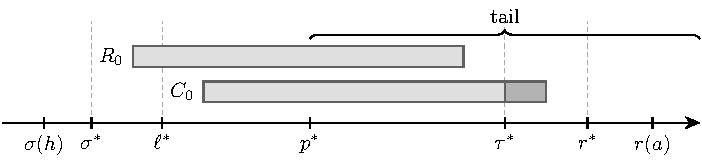
\includegraphics{positions.pdf}
    \caption{The positions in the remaining case: the ranges of $R_0$ and $C_0$, and in the dark part every class of $C_0$ has a position}
    \label{fig:positions}
\end{figure}

\emph{Property $(\star)$.}
Let $a \in R_0$ and $h \in C_0$ with $h \not\leq a$, let $\alpha$ be the position of an element of $R_0 \cap C'(h)$, and let $\beta$ be the position of an element of $C_0 \cap C(a)$.
Then the closed interval between $\alpha$ and $\beta$ contains an element of $\Pos[a] \cup \Pos[h]$.

To prove $(\star)$, we have $\alpha \neq \beta$, because $\alpha$ is the position of a high and $\beta$ of a low.
We put $p_1 = \sigma(h)$, $p_4 = r(a)$, $p_2 = \min\{\alpha, \beta\}$ and $p_3 = \max\{\alpha, \beta\}$.
By~\eqref{eq:pa-ranges-r} and~\eqref{eq:pa-ranges-c}, $p_1 \leq \sigma^*$ and $p_4 \geq r^*$.
By the same relations and $\sigma^* < \ell^*$, we have $\alpha \geq \sigma^* + 6$ and $\beta \geq \ell^* + 6 > \sigma^* + 6$, so $p_2 - p_1 \geq 6$.
By the same relations and $\tau^* < r^*$, we have $\alpha \leq \tau^* - 6 < r^* - 6$ and $\beta \leq r^* - 6$, so $p_4 - p_3 \geq 6$.
Every element of $Z = \Pos[a] \cup \Pos[h]$ is greater than $\sigma^* \geq p_1$ and less than $r^* \leq p_4$, by~\eqref{eq:pa-ranges-r}, by~\eqref{eq:pa-ranges-c} and by the orientation.
If $[p_2, p_3]$ contained no element of $Z$, then $Z \subseteq (p_1, p_2) \cup (p_3, p_4)$, and \cref{lem:pa-two} would give $12 \leq (p_2 - p_1) + (p_4 - p_3) \leq 8$.

\emph{Positions of $C_0$.}
Every class of $C_0$ has a position greater than $\tau^*$.
Indeed, let $h \in C_0$.
By~\eqref{eq:pa-ranges-c}, $\tau(h) - \sigma(h) \geq 12$, so $\Pos[h] \not\subseteq (\sigma(h), \tau(h))$ by \cref{lem:pa-one}(a) and \cref{lem:pa-basic}(b).
The elements of $\Pos[h]$ are positions of lows, so they differ from $\sigma(h)$ and $\tau(h)$.
By~\eqref{eq:pa-ranges-c} and $\sigma^* < \ell^*$, they are greater than $\sigma^* \geq \sigma(h)$.
So some element of $\Pos[h]$ is greater than $\tau(h) \geq \tau^*$.

\emph{Stage 1: the classes of $R_0$.}
Distinct classes of $R_0$ have disjoint position sets, hence distinct last positions.
Suppose that $R_0$ has at most four classes, and let $A_\kappa$ be a set of one representative per class.
Then $E^* \setminus \upp A_\kappa$ is an E-formula with $S = E_0 \cup A_\kappa$, it contains $L_P$ by $(\dagger)$ and it misses $A_P$, as required.

Otherwise, let $\kappa_1, \dots, \kappa_4$ be the first four classes of $R_0$ by last position, let $p^*$ be the last position of $\kappa_4$, and call the positions greater than $p^*$ the \emph{tail}.
The classes $\kappa_i$ have no position in the tail, and every other class of $R_0$ has its last position in the tail.
Every class of $C_0$ has a position in the tail, because $p^* \leq \tau^* - 6$ by~\eqref{eq:pa-ranges-r}.
Let $A_\kappa$ be a set of one representative per class $\kappa_i$.

Let $a_1$ and $a_2$ be the elements of $\kappa_1$ and $\kappa_4$ at their last positions, which form a far pair.
Let $S' = \win(a_1) \cup \win(a_2)$, so that $|S'| \leq 6$ by \cref{lem:pa-atoms}(c), and let
\[
F^1 = F^* \cup \FR(a_1, a_2) \cup \bigl((\EP(a_1) \cup \EP(a_2)) \setminus \upp S'\bigr).
\]
The down-set $F^1$ misses $U_P$.
Indeed, $F^*$ and $\FR(a_1, a_2)$ miss $U_P$.
The last term misses $A_P$, because an element of $S'$ lies in $\upp S'$ and any other element of $A_P$ lies outside both sets $\EP(a_i)$ by \cref{lem:pa-atoms}(c).

Let $\mathcal{C}_1$ be the set of the classes of $C_0$ not contained in $F^1$.
All elements of such a class lie outside the down-set $F^1$.
Let $g$ and $h$ be elements of a class of $\mathcal{C}_1$.
Then $g \notin \FR(a_1, a_2)$, so $g \in C(a_1) \cup C(a_2)$ by \cref{lem:pa-atoms}(a), and
\begin{equation}
\label{eq:pa-not-below}
h \not\leq a_1 \quad\text{and}\quad h \not\leq a_2.
\end{equation}
Indeed, $h < a_i$ would give $h \in \EP(a_i)$ by \cref{lem:pa-atoms}(c), and $h \notin \upp S'$ because $h \in L_P$ and $\upp S' \subseteq U_P$, hence $h \in F^1$.
The relation $h \sim a_i$ is impossible because $h \in L_P$ and $a_i \in U_P$.

\emph{Shape A: $|\mathcal{C}_1| \leq 4$.}
Let $H_1$ be a set of one representative per class of $\mathcal{C}_1$.
Then $D = F^1 \cup \dn H_1$ is an F-formula with $x_1, \dots, x_6$ equal to $a^\ell_1, a^\ell_2, a^r_1, a^r_2, a_1, a_2$, with $S = H_0 \cup H_1$ and with $S'$ as above.
It misses $U_P$ by $(\dagger)$.
It contains $B_P$, because an element of $B_P$ outside $F^1$ lies in a class of $\mathcal{C}_1$, so it is tied with an element of $H_1$.

\emph{Shape B: $|\mathcal{C}_1| \geq 5$.}
Choose five classes of $\mathcal{C}_1$ and one element of each, and call these elements $h_1, h_3, h_0, h_2, h_4$ in the order of their positions.
These positions have the same parity, so $h_1, h_2$ and $h_3, h_4$ are two far pairs, and $h_1, h_2, h_3, h_4$ lie in four distinct classes.
Let
\[
D = \bigl(E^* \cap \ER(h_1, h_2) \cap \ER(h_3, h_4)\bigr) \setminus \upp A_\kappa,
\]
which is an E-formula with $x_1, \dots, x_8$ equal to $b^\sigma_1, b^\sigma_2, b^\tau_1, b^\tau_2, h_1, h_2, h_3, h_4$ and with $S = E_0 \cup A_\kappa$.
It contains $L_P$ by \cref{lem:pa-atoms}(b) and $(\dagger)$.
We show that $D$ misses $A_P$.

Suppose that $a \in A_P \cap D$.
Then $a \in R_0$, and the class of $a$ is not among the classes $\kappa_i$.
So this class has a position in the tail, and it lies inside the down-set $D$.
Let $\Lambda$ be the set of the positions in the tail of the classes of $R_0$ inside $D$ and of the classes of $\mathcal{C}_1$.
It contains positions of highs, as just shown, and positions of lows, because every class of $C_0$ has a position in the tail.
So $\Lambda$ contains two consecutive elements $\alpha$ and $\beta$, where $\alpha$ is the position of an element $a''$ in a class of $R_0$ inside $D$, and $\beta$ is the position of an element $g$ in a class of $\mathcal{C}_1$.

At most one of the four classes of $h_1, h_2, h_3, h_4$ contains $g$, so one of the two pairs has both classes not containing $g$, and we may assume that this pair is $h_1, h_2$.
As $a'' \in D \subseteq \ER(h_1, h_2)$, \cref{lem:pa-atoms}(b) gives $h \in \{h_1, h_2\}$ with $a'' \in C'(h)$.
As $g \in C(a_1) \cup C(a_2)$, there is $a' \in \{a_1, a_2\}$ with $g \in C(a')$.
We have $a' \in R_0$, $h \in C_0$, and $h \not\leq a'$ by~\eqref{eq:pa-not-below}, so $(\star)$ applies to $a'$, $h$, $\alpha$ and $\beta$.

The closed interval between $\alpha$ and $\beta$ lies in the tail, so it misses $\Pos[a']$.
Its interior contains no element of $\Lambda$, and the class of $h$ belongs to $\mathcal{C}_1$, so its interior misses $\Pos[h]$.
Also $\alpha \notin \Pos[h]$, because $\alpha$ is the position of a high, and $\beta \notin \Pos[h]$, because the class of $h$ does not contain $g$.
This contradicts $(\star)$, so $D$ misses $A_P$.
\end{proof}

\subsection{The Algorithm}
\label{sec:pa-algorithm}

\begin{corollary}[Deciding ZZ with P2]
\label{cor:pa-zz}
There is an algorithm that, given an instance of ZZ with P2 and with $|Q| = m$, decides whether it is a yes-instance and, if it is, returns a down-set $D$ with $u \in D$ and $v \notin D$ such that $u$ and $v$ are connected in $G_D$.
Its running time is $O(m^{30})$.
\end{corollary}

\begin{proof}
For each formula of \cref{def:pa-atoms} and each choice of its elements and sets, the algorithm computes the value $D$ of the formula and tests whether $u \in D$, $v \notin D$ and $u$ and $v$ are connected in $G_D$.
It returns the first $D$ that passes the test, and it reports a no-instance if there is none.

\emph{Correctness.}
Every value is a down-set, so a returned $D$ proves a yes-instance.
Conversely, a yes-instance has a shortest valid walk $P$ by \cref{lem:zz-valid}(c), and by \cref{thm:pa-formulas} and \cref{lem:zz-valid}(a), some value passes the test.

\emph{Time.}
A choice of elements and sets of total size at most $j$ is given by a $j$-tuple over $Q$ and one extra symbol for an empty role, so there are at most $(m + 1)^j$ such choices.
Since each formula is built from at most 28 elements, there are $O(m^{28})$ tests, because $m \geq 2$.
The table of $\leq$ is given, and the sets $\MB(x)$ and $\MA(x)$ are computed once in $O(m^3)$ time.
Then each value of a formula takes $O(m^2)$ time, and a search in $G_D$ takes $O(m^2)$ time.
\end{proof}

\begin{algorithm}[tb]
\caption{A minimum cut-path for an instance $(G, u, v)$ of the open case}
\label{alg:pa-open-case}
\begin{algorithmic}[1]
\Require a graph $G \in \DC$ and vertices $u, v$ with $d(u, v) = 2$ and $c(u, v) \geq 3$
\Ensure a minimum cut-path between $u$ and $v$
\State Compute the ZZ instance $(Q, \leq, R, u, v)$ of $(G, u, v)$.
\State Run the algorithm of \cref{cor:pa-zz} on this instance.
\If{it returns a down-set $D$}
\State \Return $\delta(A)$ for a minimum side $A$ with $A \cap Q = D$
\Else
\State \Return $C \cup \pi$ for a minimum $u$--$v$ cut $C$ and a shortest $u$--$v$ path $\pi$
\EndIf
\end{algorithmic}
\end{algorithm}

\begin{theorem}[The open case]
\label{thm:pa-open-case}
There is an algorithm that, given a graph $G \in \DC$ with $n$ vertices and vertices $u, v$ of $G$ with $d(u, v) = 2$ and $c(u, v) \geq 3$, decides whether $\cp(u, v) = c(u, v)$ and computes a minimum cut-path between $u$ and $v$ in $O(n^{30})$ time.
\end{theorem}

\begin{proof}
We show that \cref{alg:pa-open-case} has these properties.
By \cref{thm:zz-reduction}, the ZZ instance satisfies P2, it has at most $n$ elements, and it is a yes-instance if and only if $\cp(u, v) = c(u, v)$.
If the algorithm of \cref{cor:pa-zz} returns $D$, then $\delta(A)$ is a minimum cut-path by \cref{thm:zz-reduction}.
Otherwise $\cp(u, v) = c(u, v) + 1$ by \cref{prop:easy-pairs}(iv), and $C \cup \pi$ has at most $c(u, v) + 1$ edges by \cref{lem:basic-bounds}, so it is a minimum cut-path.
The running time follows from \cref{thm:zz-reduction,cor:pa-zz}, since $|Q| \leq n$, and a minimum $u$--$v$ cut and a shortest $u$--$v$ path take $O(n^3)$ time.
\end{proof}

\section{Conclusion}\label{sec:conclusion}

\MinCutPath{} is NP-complete on graphs of diameter three (\cref{thm:dt-hardness}) and solvable in polynomial time on $\DC$ (\cref{thm:main}).
A pair with $c(u, v) \leq 2$ takes linear time (\cref{thm:linear-time}), and a pair with $d(u, v) = 2$ and $c(u, v) \geq 3$ takes $O(n^{30})$ time (\cref{thm:pa-open-case}).

We leave the following questions open.
\begin{enumerate}
\item Is there an algorithm with a small exponent for the pairs with $d(u, v) = 2$ and $c(u, v) \geq 3$?
The exponent $30$ comes from the $28$ elements of a formula of \cref{thm:pa-formulas}, and the algorithm does not use the structure of the formula.

\item Let $k \geq 3$ be a fixed integer, and consider the connected graphs in which every two distinct vertices $x$ and $y$ satisfy $d(x, y) \leq k$ or $c(x, y) \leq 2$.
Can $\cp(u, v)$ be computed in linear time for the pairs with $c(u, v) = 2$ in these graphs?
The paths of \cref{thm:characterization} then have at most $k$ edges, by the argument of \cref{cor:two-edges}, but the bound of four candidates per pair of terminals in \cref{alg:cut-two} uses that they have at most two.

\item Consider the connected graphs in which every two distinct vertices $x$ and $y$ satisfy $d(x, y) \leq 2$ or $c(x, y) \leq 3$.
Can $\cp(u, v)$ be computed in polynomial time for the pairs with $c(u, v) = 3$ in these graphs?
By \cref{lem:basic-bounds}, such a pair with $d(u, v) \geq 3$ has $d(u, v) \leq \cp(u, v) \leq d(u, v) + 2$, and the square decomposition is defined for cut-value two only.
\end{enumerate}

\backmatter

\bmhead{Acknowledgements}

The idea of the \MinCutPath{} problem is due to Martin Loebl, who supervised the master's thesis on which part of this paper is based.

\section*{Declarations}

\begin{itemize}
\item Funding: Statement.
\item Conflict of interest/Competing interests: Statement.
\item Ethics approval and consent to participate: Not applicable.
\item Consent for publication: Not applicable.
\item Data availability: No datasets were generated or analyzed during the current study.
\item Materials availability: Not applicable.
\item Code availability: Not applicable.
\item Author contribution: Statement.
\end{itemize}

%%===========================================================================================%%
%% If you are submitting to one of the Nature Portfolio journals, using the eJP submission   %%
%% system, please include the references within the manuscript file itself. You may do this  %%
%% by copying the reference list from your .bbl file, paste it into the main manuscript .tex %%
%% file, and delete the associated \verb+\bibliography+ commands.                            %%
%%===========================================================================================%%

\bibliography{references}% common bib file
%% if required, the content of .bbl file can be included here once bbl is generated
%%\input sn-article.bbl

\end{document}
